% Qualifying Exam Q5P1 - Optical Dynamics Modeling
% typeset with pdflatex, bibtex, pdflatex, pdflatex

\documentclass{aiaa-tc}
% % \usepackage[square,sort&compress,numbers]{natbib} % Provides formatting for
                                                  % citations
\usepackage{textcomp} % Provides math symbols that can be used in text mode
\usepackage{amssymb}  % Provides additional AMS math symbols.  Note that
                      % amsmath is loaded as part of the afit-etd class
\usepackage{bm}       % Provides bold-faced math symbols
\usepackage{booktabs} % Provides improved table formatting
\usepackage{dcolumn}  % Provides table columns aligned at decimal points
\usepackage{multirow} % Provides table elements spanning multiple rows
% \usepackage{multicol}   % ??
\usepackage{graphicx} % Standard package to incorporate graphics
\usepackage[printonlyused]{acronym} % Provides a method for incorporating
                                    % acronyms and building an acronym list
\usepackage{subfigure} % Create subfigures
\usepackage{subfig}
\usepackage{calc}      % allows simple and easy calculations
\usepackage{wrapfig}   % wrapped text around figures - perhaps not appropriate
                       % in a thesis, but useful in general
% \usepackage[numbered]{mcode} % easily integrates matlab code
\usepackage{float} %H places the figure or tables in that exact location
\usepackage{amsthm}
\newtheorem*{definition}{Definition}
\usepackage{pdfpages}
\usepackage{subfigure} % Create subfigures
\usepackage{float} %H places the figure or tables in that exact location
\usepackage{multirow}
\usepackage{longtable}
\usepackage{tabu}
\usepackage{tikz}
% \usepackage{caption}
% \usepackage{subcaption}


%\usepackage{ifpdf} % \ifpdf ... \else ... fi structure
%\ifpdf 
%  \usepackage[pdftex, bookmarks, breaklinks,
%              plainpages=false,% Make page anchors using the formatted form of 
%                               % the page number. With this option, hyperref 
%                               % writes different anchors for pages 'ii' and
%                               % '2'. (If the option is set 'true' - the 
%                               % default - hyperref writes page anchors as the
%                               % arabic form of the absolute page number, 
%                               % rather than the formatted form.) [UK TeXfaq]
%              pdfpagelabels,   % Set PDF page labels; i.e., write the
%                               % value of \thepage to the PDF file so that
%                               % Acrobat Reader can display the page number as
%                               % (say) 'ii (4 of 40)' rather than simply '4 of
%                               % 40'. [UK TeXfaq]
%              colorlinks,      % use color instead of boxes for links
%              linkcolor=black, % color internal links black
%              urlcolor=black,  % color url's black
%              citecolor=black, % color links to references black
%              ]{hyperref} 
%\else  
%  \usepackage[hypertex]{hyperref}
%\fi

\usepackage{subfigure} % Create subfigures
\usepackage{float} %H places the figure or tables in that exact location
\usepackage{multirow}
\usepackage{longtable}
\usepackage{tabu}
\usepackage{tikz}
\usetikzlibrary{calc,patterns,decorations.pathmorphing,decorations.markings}
\usepackage{amsmath}
\usepackage{amssymb}
\usepackage{array}
\usepackage{graphicx}
\usepackage{epstopdf}
\usepackage{bigints}

\title{COON - Qualifying Exam Q5, P1}

\author{Timothy E. Coon\thanks{PhD Student, Department of Aeronautics and Astronautics, 2950 Hobson Way} \\
%EndAName
{\normalsize \itshape Air Force Institute of Technology, Wright-Patterson AFB, OH, 45433}\\}

% Macros for Scientific Word 4.0 documents saved with the LaTeX filter.
% Copyright (C) 2002 Mackichan Software, Inc.

\typeout{TCILATEX Macros for Scientific Word 5.0 <13 Feb 2003>.}
\typeout{NOTICE:  This macro file is NOT proprietary and may be 
freely copied and distributed.}
%
\makeatletter

%%%%%%%%%%%%%%%%%%%%%
% pdfTeX related.
\ifx\pdfoutput\relax\let\pdfoutput=\undefined\fi
\newcount\msipdfoutput
\ifx\pdfoutput\undefined
\else
 \ifcase\pdfoutput
 \else 
    \msipdfoutput=1
    \ifx\paperwidth\undefined
    \else
      \ifdim\paperheight=0pt\relax
      \else
        \pdfpageheight\paperheight
      \fi
      \ifdim\paperwidth=0pt\relax
      \else
        \pdfpagewidth\paperwidth
      \fi
    \fi
  \fi  
\fi

%%%%%%%%%%%%%%%%%%%%%
% FMTeXButton
% This is used for putting TeXButtons in the 
% frontmatter of a document. Add a line like
% \QTagDef{FMTeXButton}{101}{} to the filter 
% section of the cst being used. Also add a
% new section containing:
%     [f_101]
%     ALIAS=FMTexButton
%     TAG_TYPE=FIELD
%     TAG_LEADIN=TeX Button:
%
% It also works to put \defs in the preamble after 
% the \input tcilatex
\def\FMTeXButton#1{#1}
%
%%%%%%%%%%%%%%%%%%%%%%
% macros for time
\newcount\@hour\newcount\@minute\chardef\@x10\chardef\@xv60
\def\tcitime{
\def\@time{%
  \@minute\time\@hour\@minute\divide\@hour\@xv
  \ifnum\@hour<\@x 0\fi\the\@hour:%
  \multiply\@hour\@xv\advance\@minute-\@hour
  \ifnum\@minute<\@x 0\fi\the\@minute
  }}%

%%%%%%%%%%%%%%%%%%%%%%
% macro for hyperref and msihyperref
%\@ifundefined{hyperref}{\def\hyperref#1#2#3#4{#2\ref{#4}#3}}{}

\def\x@hyperref#1#2#3{%
   % Turn off various catcodes before reading parameter 4
   \catcode`\~ = 12
   \catcode`\$ = 12
   \catcode`\_ = 12
   \catcode`\# = 12
   \catcode`\& = 12
   \catcode`\% = 12
   \y@hyperref{#1}{#2}{#3}%
}

\def\y@hyperref#1#2#3#4{%
   #2\ref{#4}#3
   \catcode`\~ = 13
   \catcode`\$ = 3
   \catcode`\_ = 8
   \catcode`\# = 6
   \catcode`\& = 4
   \catcode`\% = 14
}

\@ifundefined{hyperref}{\let\hyperref\x@hyperref}{}
\@ifundefined{msihyperref}{\let\msihyperref\x@hyperref}{}




% macro for external program call
\@ifundefined{qExtProgCall}{\def\qExtProgCall#1#2#3#4#5#6{\relax}}{}
%%%%%%%%%%%%%%%%%%%%%%
%
% macros for graphics
%
\def\FILENAME#1{#1}%
%
\def\QCTOpt[#1]#2{%
  \def\QCTOptB{#1}
  \def\QCTOptA{#2}
}
\def\QCTNOpt#1{%
  \def\QCTOptA{#1}
  \let\QCTOptB\empty
}
\def\Qct{%
  \@ifnextchar[{%
    \QCTOpt}{\QCTNOpt}
}
\def\QCBOpt[#1]#2{%
  \def\QCBOptB{#1}%
  \def\QCBOptA{#2}%
}
\def\QCBNOpt#1{%
  \def\QCBOptA{#1}%
  \let\QCBOptB\empty
}
\def\Qcb{%
  \@ifnextchar[{%
    \QCBOpt}{\QCBNOpt}%
}
\def\PrepCapArgs{%
  \ifx\QCBOptA\empty
    \ifx\QCTOptA\empty
      {}%
    \else
      \ifx\QCTOptB\empty
        {\QCTOptA}%
      \else
        [\QCTOptB]{\QCTOptA}%
      \fi
    \fi
  \else
    \ifx\QCBOptA\empty
      {}%
    \else
      \ifx\QCBOptB\empty
        {\QCBOptA}%
      \else
        [\QCBOptB]{\QCBOptA}%
      \fi
    \fi
  \fi
}
\newcount\GRAPHICSTYPE
%\GRAPHICSTYPE 0 is for TurboTeX
%\GRAPHICSTYPE 1 is for DVIWindo (PostScript)
%%%(removed)%\GRAPHICSTYPE 2 is for psfig (PostScript)
\GRAPHICSTYPE=\z@
\def\GRAPHICSPS#1{%
 \ifcase\GRAPHICSTYPE%\GRAPHICSTYPE=0
   \special{ps: #1}%
 \or%\GRAPHICSTYPE=1
   \special{language "PS", include "#1"}%
%%%\or%\GRAPHICSTYPE=2
%%%  #1%
 \fi
}%
%
\def\GRAPHICSHP#1{\special{include #1}}%
%
% \graffile{ body }                                  %#1
%          { contentswidth (scalar)  }               %#2
%          { contentsheight (scalar) }               %#3
%          { vertical shift when in-line (scalar) }  %#4

\def\graffile#1#2#3#4{%
%%% \ifnum\GRAPHICSTYPE=\tw@
%%%  %Following if using psfig
%%%  \@ifundefined{psfig}{\input psfig.tex}{}%
%%%  \psfig{file=#1, height=#3, width=#2}%
%%% \else
  %Following for all others
  % JCS - added BOXTHEFRAME, see below
    \bgroup
	   \@inlabelfalse
       \leavevmode
       \@ifundefined{bbl@deactivate}{\def~{\string~}}{\activesoff}%
        \raise -#4 \BOXTHEFRAME{%
           \hbox to #2{\raise #3\hbox to #2{\null #1\hfil}}}%
    \egroup
}%
%
% A box for drafts
\def\draftbox#1#2#3#4{%
 \leavevmode\raise -#4 \hbox{%
  \frame{\rlap{\protect\tiny #1}\hbox to #2%
   {\vrule height#3 width\z@ depth\z@\hfil}%
  }%
 }%
}%
%
\newcount\@msidraft
\@msidraft=\z@
\let\nographics=\@msidraft
\newif\ifwasdraft
\wasdraftfalse

%  \GRAPHIC{ body }                                  %#1
%          { draft name }                            %#2
%          { contentswidth (scalar)  }               %#3
%          { contentsheight (scalar) }               %#4
%          { vertical shift when in-line (scalar) }  %#5
\def\GRAPHIC#1#2#3#4#5{%
   \ifnum\@msidraft=\@ne\draftbox{#2}{#3}{#4}{#5}%
   \else\graffile{#1}{#3}{#4}{#5}%
   \fi
}
%
\def\addtoLaTeXparams#1{%
    \edef\LaTeXparams{\LaTeXparams #1}}%
%
% JCS -  added a switch BoxFrame that can 
% be set by including X in the frame params.
% If set a box is drawn around the frame.

\newif\ifBoxFrame \BoxFramefalse
\newif\ifOverFrame \OverFramefalse
\newif\ifUnderFrame \UnderFramefalse

\def\BOXTHEFRAME#1{%
   \hbox{%
      \ifBoxFrame
         \frame{#1}%
      \else
         {#1}%
      \fi
   }%
}


\def\doFRAMEparams#1{\BoxFramefalse\OverFramefalse\UnderFramefalse\readFRAMEparams#1\end}%
\def\readFRAMEparams#1{%
 \ifx#1\end%
  \let\next=\relax
  \else
  \ifx#1i\dispkind=\z@\fi
  \ifx#1d\dispkind=\@ne\fi
  \ifx#1f\dispkind=\tw@\fi
  \ifx#1t\addtoLaTeXparams{t}\fi
  \ifx#1b\addtoLaTeXparams{b}\fi
  \ifx#1p\addtoLaTeXparams{p}\fi
  \ifx#1h\addtoLaTeXparams{h}\fi
  \ifx#1X\BoxFrametrue\fi
  \ifx#1O\OverFrametrue\fi
  \ifx#1U\UnderFrametrue\fi
  \ifx#1w
    \ifnum\@msidraft=1\wasdrafttrue\else\wasdraftfalse\fi
    \@msidraft=\@ne
  \fi
  \let\next=\readFRAMEparams
  \fi
 \next
 }%
%
%Macro for In-line graphics object
%   \IFRAME{ contentswidth (scalar)  }               %#1
%          { contentsheight (scalar) }               %#2
%          { vertical shift when in-line (scalar) }  %#3
%          { draft name }                            %#4
%          { body }                                  %#5
%          { caption}                                %#6


\def\IFRAME#1#2#3#4#5#6{%
      \bgroup
      \let\QCTOptA\empty
      \let\QCTOptB\empty
      \let\QCBOptA\empty
      \let\QCBOptB\empty
      #6%
      \parindent=0pt
      \leftskip=0pt
      \rightskip=0pt
      \setbox0=\hbox{\QCBOptA}%
      \@tempdima=#1\relax
      \ifOverFrame
          % Do this later
          \typeout{This is not implemented yet}%
          \show\HELP
      \else
         \ifdim\wd0>\@tempdima
            \advance\@tempdima by \@tempdima
            \ifdim\wd0 >\@tempdima
               \setbox1 =\vbox{%
                  \unskip\hbox to \@tempdima{\hfill\GRAPHIC{#5}{#4}{#1}{#2}{#3}\hfill}%
                  \unskip\hbox to \@tempdima{\parbox[b]{\@tempdima}{\QCBOptA}}%
               }%
               \wd1=\@tempdima
            \else
               \textwidth=\wd0
               \setbox1 =\vbox{%
                 \noindent\hbox to \wd0{\hfill\GRAPHIC{#5}{#4}{#1}{#2}{#3}\hfill}\\%
                 \noindent\hbox{\QCBOptA}%
               }%
               \wd1=\wd0
            \fi
         \else
            \ifdim\wd0>0pt
              \hsize=\@tempdima
              \setbox1=\vbox{%
                \unskip\GRAPHIC{#5}{#4}{#1}{#2}{0pt}%
                \break
                \unskip\hbox to \@tempdima{\hfill \QCBOptA\hfill}%
              }%
              \wd1=\@tempdima
           \else
              \hsize=\@tempdima
              \setbox1=\vbox{%
                \unskip\GRAPHIC{#5}{#4}{#1}{#2}{0pt}%
              }%
              \wd1=\@tempdima
           \fi
         \fi
         \@tempdimb=\ht1
         %\advance\@tempdimb by \dp1
         \advance\@tempdimb by -#2
         \advance\@tempdimb by #3
         \leavevmode
         \raise -\@tempdimb \hbox{\box1}%
      \fi
      \egroup%
}%
%
%Macro for Display graphics object
%   \DFRAME{ contentswidth (scalar)  }               %#1
%          { contentsheight (scalar) }               %#2
%          { draft label }                           %#3
%          { name }                                  %#4
%          { caption}                                %#5
\def\DFRAME#1#2#3#4#5{%
  \vspace\topsep
  \hfil\break
  \bgroup
     \leftskip\@flushglue
	 \rightskip\@flushglue
	 \parindent\z@
	 \parfillskip\z@skip
     \let\QCTOptA\empty
     \let\QCTOptB\empty
     \let\QCBOptA\empty
     \let\QCBOptB\empty
	 \vbox\bgroup
        \ifOverFrame 
           #5\QCTOptA\par
        \fi
        \GRAPHIC{#4}{#3}{#1}{#2}{\z@}%
        \ifUnderFrame 
           \break#5\QCBOptA
        \fi
	 \egroup
  \egroup
  \vspace\topsep
  \break
}%
%
%Macro for Floating graphic object
%   \FFRAME{ framedata f|i tbph x F|T }              %#1
%          { contentswidth (scalar)  }               %#2
%          { contentsheight (scalar) }               %#3
%          { caption }                               %#4
%          { label }                                 %#5
%          { draft name }                            %#6
%          { body }                                  %#7
\def\FFRAME#1#2#3#4#5#6#7{%
 %If float.sty loaded and float option is 'h', change to 'H'  (gp) 1998/09/05
  \@ifundefined{floatstyle}
    {%floatstyle undefined (and float.sty not present), no change
     \begin{figure}[#1]%
    }
    {%floatstyle DEFINED
	 \ifx#1h%Only the h parameter, change to H
      \begin{figure}[H]%
	 \else
      \begin{figure}[#1]%
	 \fi
	}
  \let\QCTOptA\empty
  \let\QCTOptB\empty
  \let\QCBOptA\empty
  \let\QCBOptB\empty
  \ifOverFrame
    #4
    \ifx\QCTOptA\empty
    \else
      \ifx\QCTOptB\empty
        \caption{\QCTOptA}%
      \else
        \caption[\QCTOptB]{\QCTOptA}%
      \fi
    \fi
    \ifUnderFrame\else
      \label{#5}%
    \fi
  \else
    \UnderFrametrue%
  \fi
  \begin{center}\GRAPHIC{#7}{#6}{#2}{#3}{\z@}\end{center}%
  \ifUnderFrame
    #4
    \ifx\QCBOptA\empty
      \caption{}%
    \else
      \ifx\QCBOptB\empty
        \caption{\QCBOptA}%
      \else
        \caption[\QCBOptB]{\QCBOptA}%
      \fi
    \fi
    \label{#5}%
  \fi
  \end{figure}%
 }%
%
%
%    \FRAME{ framedata f|i tbph x F|T }              %#1
%          { contentswidth (scalar)  }               %#2
%          { contentsheight (scalar) }               %#3
%          { vertical shift when in-line (scalar) }  %#4
%          { caption }                               %#5
%          { label }                                 %#6
%          { name }                                  %#7
%          { body }                                  %#8
%
%    framedata is a string which can contain the following
%    characters: idftbphxFT
%    Their meaning is as follows:
%             i, d or f : in-line, display, or floating
%             t,b,p,h   : LaTeX floating placement options
%             x         : fit contents box to contents
%             F or T    : Figure or Table. 
%                         Later this can expand
%                         to a more general float class.
%
%
\newcount\dispkind%

\def\makeactives{
  \catcode`\"=\active
  \catcode`\;=\active
  \catcode`\:=\active
  \catcode`\'=\active
  \catcode`\~=\active
}
\bgroup
   \makeactives
   \gdef\activesoff{%
      \def"{\string"}%
      \def;{\string;}%
      \def:{\string:}%
      \def'{\string'}%
      \def~{\string~}%
      %\bbl@deactivate{"}%
      %\bbl@deactivate{;}%
      %\bbl@deactivate{:}%
      %\bbl@deactivate{'}%
    }
\egroup

\def\FRAME#1#2#3#4#5#6#7#8{%
 \bgroup
 \ifnum\@msidraft=\@ne
   \wasdrafttrue
 \else
   \wasdraftfalse%
 \fi
 \def\LaTeXparams{}%
 \dispkind=\z@
 \def\LaTeXparams{}%
 \doFRAMEparams{#1}%
 \ifnum\dispkind=\z@\IFRAME{#2}{#3}{#4}{#7}{#8}{#5}\else
  \ifnum\dispkind=\@ne\DFRAME{#2}{#3}{#7}{#8}{#5}\else
   \ifnum\dispkind=\tw@
    \edef\@tempa{\noexpand\FFRAME{\LaTeXparams}}%
    \@tempa{#2}{#3}{#5}{#6}{#7}{#8}%
    \fi
   \fi
  \fi
  \ifwasdraft\@msidraft=1\else\@msidraft=0\fi{}%
  \egroup
 }%
%
% This macro added to let SW gobble a parameter that
% should not be passed on and expanded. 

\def\TEXUX#1{"texux"}

%
% Macros for text attributes:
%
\def\BF#1{{\bf {#1}}}%
\def\NEG#1{\leavevmode\hbox{\rlap{\thinspace/}{$#1$}}}%
%
%%%%%%%%%%%%%%%%%%%%%%%%%%%%%%%%%%%%%%%%%%%%%%%%%%%%%%%%%%%%%%%%%%%%%%%%
%
%
% macros for user - defined functions
\def\limfunc#1{\mathop{\rm #1}}%
\def\func#1{\mathop{\rm #1}\nolimits}%
% macro for unit names
\def\unit#1{\mathord{\thinspace\rm #1}}%

%
% miscellaneous 
\long\def\QQQ#1#2{%
     \long\expandafter\def\csname#1\endcsname{#2}}%
\@ifundefined{QTP}{\def\QTP#1{}}{}
\@ifundefined{QEXCLUDE}{\def\QEXCLUDE#1{}}{}
\@ifundefined{Qlb}{\def\Qlb#1{#1}}{}
\@ifundefined{Qlt}{\def\Qlt#1{#1}}{}
\def\QWE{}%
\long\def\QQA#1#2{}%
\def\QTR#1#2{{\csname#1\endcsname {#2}}}%
\long\def\TeXButton#1#2{#2}%
\long\def\QSubDoc#1#2{#2}%
\def\EXPAND#1[#2]#3{}%
\def\NOEXPAND#1[#2]#3{}%
\def\PROTECTED{}%
\def\LaTeXparent#1{}%
\def\ChildStyles#1{}%
\def\ChildDefaults#1{}%
\def\QTagDef#1#2#3{}%

% Constructs added with Scientific Notebook
\@ifundefined{correctchoice}{\def\correctchoice{\relax}}{}
\@ifundefined{HTML}{\def\HTML#1{\relax}}{}
\@ifundefined{TCIIcon}{\def\TCIIcon#1#2#3#4{\relax}}{}
\if@compatibility
  \typeout{Not defining UNICODE  U or CustomNote commands for LaTeX 2.09.}
\else
  \providecommand{\UNICODE}[2][]{\protect\rule{.1in}{.1in}}
  \providecommand{\U}[1]{\protect\rule{.1in}{.1in}}
  \providecommand{\CustomNote}[3][]{\marginpar{#3}}
\fi

\@ifundefined{lambdabar}{
      \def\lambdabar{\errmessage{You have used the lambdabar symbol. 
                      This is available for typesetting only in RevTeX styles.}}
   }{}

%
% Macros for style editor docs
\@ifundefined{StyleEditBeginDoc}{\def\StyleEditBeginDoc{\relax}}{}
%
% Macros for footnotes
\def\QQfnmark#1{\footnotemark}
\def\QQfntext#1#2{\addtocounter{footnote}{#1}\footnotetext{#2}}
%
% Macros for indexing.
%
\@ifundefined{TCIMAKEINDEX}{}{\makeindex}%
%
% Attempts to avoid problems with other styles
\@ifundefined{abstract}{%
 \def\abstract{%
  \if@twocolumn
   \section*{Abstract (Not appropriate in this style!)}%
   \else \small 
   \begin{center}{\bf Abstract\vspace{-.5em}\vspace{\z@}}\end{center}%
   \quotation 
   \fi
  }%
 }{%
 }%
\@ifundefined{endabstract}{\def\endabstract
  {\if@twocolumn\else\endquotation\fi}}{}%
\@ifundefined{maketitle}{\def\maketitle#1{}}{}%
\@ifundefined{affiliation}{\def\affiliation#1{}}{}%
\@ifundefined{proof}{\def\proof{\noindent{\bfseries Proof. }}}{}%
\@ifundefined{endproof}{\def\endproof{\mbox{\ \rule{.1in}{.1in}}}}{}%
\@ifundefined{newfield}{\def\newfield#1#2{}}{}%
\@ifundefined{chapter}{\def\chapter#1{\par(Chapter head:)#1\par }%
 \newcount\c@chapter}{}%
\@ifundefined{part}{\def\part#1{\par(Part head:)#1\par }}{}%
\@ifundefined{section}{\def\section#1{\par(Section head:)#1\par }}{}%
\@ifundefined{subsection}{\def\subsection#1%
 {\par(Subsection head:)#1\par }}{}%
\@ifundefined{subsubsection}{\def\subsubsection#1%
 {\par(Subsubsection head:)#1\par }}{}%
\@ifundefined{paragraph}{\def\paragraph#1%
 {\par(Subsubsubsection head:)#1\par }}{}%
\@ifundefined{subparagraph}{\def\subparagraph#1%
 {\par(Subsubsubsubsection head:)#1\par }}{}%
%%%%%%%%%%%%%%%%%%%%%%%%%%%%%%%%%%%%%%%%%%%%%%%%%%%%%%%%%%%%%%%%%%%%%%%%
% These symbols are not recognized by LaTeX
\@ifundefined{therefore}{\def\therefore{}}{}%
\@ifundefined{backepsilon}{\def\backepsilon{}}{}%
\@ifundefined{yen}{\def\yen{\hbox{\rm\rlap=Y}}}{}%
\@ifundefined{registered}{%
   \def\registered{\relax\ifmmode{}\r@gistered
                    \else$\m@th\r@gistered$\fi}%
 \def\r@gistered{^{\ooalign
  {\hfil\raise.07ex\hbox{$\scriptstyle\rm\text{R}$}\hfil\crcr
  \mathhexbox20D}}}}{}%
\@ifundefined{Eth}{\def\Eth{}}{}%
\@ifundefined{eth}{\def\eth{}}{}%
\@ifundefined{Thorn}{\def\Thorn{}}{}%
\@ifundefined{thorn}{\def\thorn{}}{}%
% A macro to allow any symbol that requires math to appear in text
\def\TEXTsymbol#1{\mbox{$#1$}}%
\@ifundefined{degree}{\def\degree{{}^{\circ}}}{}%
%
% macros for T3TeX files
\newdimen\theight
\@ifundefined{Column}{\def\Column{%
 \vadjust{\setbox\z@=\hbox{\scriptsize\quad\quad tcol}%
  \theight=\ht\z@\advance\theight by \dp\z@\advance\theight by \lineskip
  \kern -\theight \vbox to \theight{%
   \rightline{\rlap{\box\z@}}%
   \vss
   }%
  }%
 }}{}%
%
\@ifundefined{qed}{\def\qed{%
 \ifhmode\unskip\nobreak\fi\ifmmode\ifinner\else\hskip5\p@\fi\fi
 \hbox{\hskip5\p@\vrule width4\p@ height6\p@ depth1.5\p@\hskip\p@}%
 }}{}%
%
\@ifundefined{cents}{\def\cents{\hbox{\rm\rlap c/}}}{}%
\@ifundefined{tciLaplace}{\def\tciLaplace{\ensuremath{\mathcal{L}}}}{}%
\@ifundefined{tciFourier}{\def\tciFourier{\ensuremath{\mathcal{F}}}}{}%
\@ifundefined{textcurrency}{\def\textcurrency{\hbox{\rm\rlap xo}}}{}%
\@ifundefined{texteuro}{\def\texteuro{\hbox{\rm\rlap C=}}}{}%
\@ifundefined{euro}{\def\euro{\hbox{\rm\rlap C=}}}{}%
\@ifundefined{textfranc}{\def\textfranc{\hbox{\rm\rlap-F}}}{}%
\@ifundefined{textlira}{\def\textlira{\hbox{\rm\rlap L=}}}{}%
\@ifundefined{textpeseta}{\def\textpeseta{\hbox{\rm P\negthinspace s}}}{}%
%
\@ifundefined{miss}{\def\miss{\hbox{\vrule height2\p@ width 2\p@ depth\z@}}}{}%
%
\@ifundefined{vvert}{\def\vvert{\Vert}}{}%  %always translated to \left| or \right|
%
\@ifundefined{tcol}{\def\tcol#1{{\baselineskip=6\p@ \vcenter{#1}} \Column}}{}%
%
\@ifundefined{dB}{\def\dB{\hbox{{}}}}{}%        %dummy entry in column 
\@ifundefined{mB}{\def\mB#1{\hbox{$#1$}}}{}%   %column entry
\@ifundefined{nB}{\def\nB#1{\hbox{#1}}}{}%     %column entry (not math)
%
\@ifundefined{note}{\def\note{$^{\dag}}}{}%
%
\def\newfmtname{LaTeX2e}
% No longer load latexsym.  This is now handled by SWP, which uses amsfonts if necessary
%
\ifx\fmtname\newfmtname
  \DeclareOldFontCommand{\rm}{\normalfont\rmfamily}{\mathrm}
  \DeclareOldFontCommand{\sf}{\normalfont\sffamily}{\mathsf}
  \DeclareOldFontCommand{\tt}{\normalfont\ttfamily}{\mathtt}
  \DeclareOldFontCommand{\bf}{\normalfont\bfseries}{\mathbf}
  \DeclareOldFontCommand{\it}{\normalfont\itshape}{\mathit}
  \DeclareOldFontCommand{\sl}{\normalfont\slshape}{\@nomath\sl}
  \DeclareOldFontCommand{\sc}{\normalfont\scshape}{\@nomath\sc}
\fi

%
% Greek bold macros
% Redefine all of the math symbols 
% which might be bolded	 - there are 
% probably others to add to this list

\def\alpha{{\Greekmath 010B}}%
\def\beta{{\Greekmath 010C}}%
\def\gamma{{\Greekmath 010D}}%
\def\delta{{\Greekmath 010E}}%
\def\epsilon{{\Greekmath 010F}}%
\def\zeta{{\Greekmath 0110}}%
\def\eta{{\Greekmath 0111}}%
\def\theta{{\Greekmath 0112}}%
\def\iota{{\Greekmath 0113}}%
\def\kappa{{\Greekmath 0114}}%
\def\lambda{{\Greekmath 0115}}%
\def\mu{{\Greekmath 0116}}%
\def\nu{{\Greekmath 0117}}%
\def\xi{{\Greekmath 0118}}%
\def\pi{{\Greekmath 0119}}%
\def\rho{{\Greekmath 011A}}%
\def\sigma{{\Greekmath 011B}}%
\def\tau{{\Greekmath 011C}}%
\def\upsilon{{\Greekmath 011D}}%
\def\phi{{\Greekmath 011E}}%
\def\chi{{\Greekmath 011F}}%
\def\psi{{\Greekmath 0120}}%
\def\omega{{\Greekmath 0121}}%
\def\varepsilon{{\Greekmath 0122}}%
\def\vartheta{{\Greekmath 0123}}%
\def\varpi{{\Greekmath 0124}}%
\def\varrho{{\Greekmath 0125}}%
\def\varsigma{{\Greekmath 0126}}%
\def\varphi{{\Greekmath 0127}}%

\def\nabla{{\Greekmath 0272}}
\def\FindBoldGroup{%
   {\setbox0=\hbox{$\mathbf{x\global\edef\theboldgroup{\the\mathgroup}}$}}%
}

\def\Greekmath#1#2#3#4{%
    \if@compatibility
        \ifnum\mathgroup=\symbold
           \mathchoice{\mbox{\boldmath$\displaystyle\mathchar"#1#2#3#4$}}%
                      {\mbox{\boldmath$\textstyle\mathchar"#1#2#3#4$}}%
                      {\mbox{\boldmath$\scriptstyle\mathchar"#1#2#3#4$}}%
                      {\mbox{\boldmath$\scriptscriptstyle\mathchar"#1#2#3#4$}}%
        \else
           \mathchar"#1#2#3#4% 
        \fi 
    \else 
        \FindBoldGroup
        \ifnum\mathgroup=\theboldgroup % For 2e
           \mathchoice{\mbox{\boldmath$\displaystyle\mathchar"#1#2#3#4$}}%
                      {\mbox{\boldmath$\textstyle\mathchar"#1#2#3#4$}}%
                      {\mbox{\boldmath$\scriptstyle\mathchar"#1#2#3#4$}}%
                      {\mbox{\boldmath$\scriptscriptstyle\mathchar"#1#2#3#4$}}%
        \else
           \mathchar"#1#2#3#4% 
        \fi     	    
	  \fi}

\newif\ifGreekBold  \GreekBoldfalse
\let\SAVEPBF=\pbf
\def\pbf{\GreekBoldtrue\SAVEPBF}%
%

\@ifundefined{theorem}{\newtheorem{theorem}{Theorem}}{}
\@ifundefined{lemma}{\newtheorem{lemma}[theorem]{Lemma}}{}
\@ifundefined{corollary}{\newtheorem{corollary}[theorem]{Corollary}}{}
\@ifundefined{conjecture}{\newtheorem{conjecture}[theorem]{Conjecture}}{}
\@ifundefined{proposition}{\newtheorem{proposition}[theorem]{Proposition}}{}
\@ifundefined{axiom}{\newtheorem{axiom}{Axiom}}{}
\@ifundefined{remark}{\newtheorem{remark}{Remark}}{}
\@ifundefined{example}{\newtheorem{example}{Example}}{}
\@ifundefined{exercise}{\newtheorem{exercise}{Exercise}}{}
\@ifundefined{definition}{\newtheorem{definition}{Definition}}{}


\@ifundefined{mathletters}{%
  %\def\theequation{\arabic{equation}}
  \newcounter{equationnumber}  
  \def\mathletters{%
     \addtocounter{equation}{1}
     \edef\@currentlabel{\theequation}%
     \setcounter{equationnumber}{\c@equation}
     \setcounter{equation}{0}%
     \edef\theequation{\@currentlabel\noexpand\alph{equation}}%
  }
  \def\endmathletters{%
     \setcounter{equation}{\value{equationnumber}}%
  }
}{}

%Logos
\@ifundefined{BibTeX}{%
    \def\BibTeX{{\rm B\kern-.05em{\sc i\kern-.025em b}\kern-.08em
                 T\kern-.1667em\lower.7ex\hbox{E}\kern-.125emX}}}{}%
\@ifundefined{AmS}%
    {\def\AmS{{\protect\usefont{OMS}{cmsy}{m}{n}%
                A\kern-.1667em\lower.5ex\hbox{M}\kern-.125emS}}}{}%
\@ifundefined{AmSTeX}{\def\AmSTeX{\protect\AmS-\protect\TeX\@}}{}%
%

% This macro is a fix to eqnarray
\def\@@eqncr{\let\@tempa\relax
    \ifcase\@eqcnt \def\@tempa{& & &}\or \def\@tempa{& &}%
      \else \def\@tempa{&}\fi
     \@tempa
     \if@eqnsw
        \iftag@
           \@taggnum
        \else
           \@eqnnum\stepcounter{equation}%
        \fi
     \fi
     \global\tag@false
     \global\@eqnswtrue
     \global\@eqcnt\z@\cr}


\def\TCItag{\@ifnextchar*{\@TCItagstar}{\@TCItag}}
\def\@TCItag#1{%
    \global\tag@true
    \global\def\@taggnum{(#1)}%
    \global\def\@currentlabel{#1}}
\def\@TCItagstar*#1{%
    \global\tag@true
    \global\def\@taggnum{#1}%
    \global\def\@currentlabel{#1}}
%
%%%%%%%%%%%%%%%%%%%%%%%%%%%%%%%%%%%%%%%%%%%%%%%%%%%%%%%%%%%%%%%%%%%%%
%
\def\QATOP#1#2{{#1 \atop #2}}%
\def\QTATOP#1#2{{\textstyle {#1 \atop #2}}}%
\def\QDATOP#1#2{{\displaystyle {#1 \atop #2}}}%
\def\QABOVE#1#2#3{{#2 \above#1 #3}}%
\def\QTABOVE#1#2#3{{\textstyle {#2 \above#1 #3}}}%
\def\QDABOVE#1#2#3{{\displaystyle {#2 \above#1 #3}}}%
\def\QOVERD#1#2#3#4{{#3 \overwithdelims#1#2 #4}}%
\def\QTOVERD#1#2#3#4{{\textstyle {#3 \overwithdelims#1#2 #4}}}%
\def\QDOVERD#1#2#3#4{{\displaystyle {#3 \overwithdelims#1#2 #4}}}%
\def\QATOPD#1#2#3#4{{#3 \atopwithdelims#1#2 #4}}%
\def\QTATOPD#1#2#3#4{{\textstyle {#3 \atopwithdelims#1#2 #4}}}%
\def\QDATOPD#1#2#3#4{{\displaystyle {#3 \atopwithdelims#1#2 #4}}}%
\def\QABOVED#1#2#3#4#5{{#4 \abovewithdelims#1#2#3 #5}}%
\def\QTABOVED#1#2#3#4#5{{\textstyle 
   {#4 \abovewithdelims#1#2#3 #5}}}%
\def\QDABOVED#1#2#3#4#5{{\displaystyle 
   {#4 \abovewithdelims#1#2#3 #5}}}%
%
% Macros for text size operators:
%

\def\tint{\msi@int\textstyle\int}%
\def\tiint{\msi@int\textstyle\iint}%
\def\tiiint{\msi@int\textstyle\iiint}%
\def\tiiiint{\msi@int\textstyle\iiiint}%
\def\tidotsint{\msi@int\textstyle\idotsint}%
\def\toint{\msi@int\textstyle\oint}%


\def\tsum{\mathop{\textstyle \sum }}%
\def\tprod{\mathop{\textstyle \prod }}%
\def\tbigcap{\mathop{\textstyle \bigcap }}%
\def\tbigwedge{\mathop{\textstyle \bigwedge }}%
\def\tbigoplus{\mathop{\textstyle \bigoplus }}%
\def\tbigodot{\mathop{\textstyle \bigodot }}%
\def\tbigsqcup{\mathop{\textstyle \bigsqcup }}%
\def\tcoprod{\mathop{\textstyle \coprod }}%
\def\tbigcup{\mathop{\textstyle \bigcup }}%
\def\tbigvee{\mathop{\textstyle \bigvee }}%
\def\tbigotimes{\mathop{\textstyle \bigotimes }}%
\def\tbiguplus{\mathop{\textstyle \biguplus }}%
%
%
%Macros for display size operators:
%

\newtoks\temptoksa
\newtoks\temptoksb
\newtoks\temptoksc


\def\msi@int#1#2{%
 \def\@temp{{#1#2\the\temptoksc_{\the\temptoksa}^{\the\temptoksb}}}%   
 \futurelet\@nextcs
 \@int
}

\def\@int{%
   \ifx\@nextcs\limits
      \typeout{Found limits}%
      \temptoksc={\limits}%
	  \let\@next\@intgobble%
   \else\ifx\@nextcs\nolimits
      \typeout{Found nolimits}%
      \temptoksc={\nolimits}%
	  \let\@next\@intgobble%
   \else
      \typeout{Did not find limits or no limits}%
      \temptoksc={}%
      \let\@next\msi@limits%
   \fi\fi
   \@next   
}%

\def\@intgobble#1{%
   \typeout{arg is #1}%
   \msi@limits
}


\def\msi@limits{%
   \temptoksa={}%
   \temptoksb={}%
   \@ifnextchar_{\@limitsa}{\@limitsb}%
}

\def\@limitsa_#1{%
   \temptoksa={#1}%
   \@ifnextchar^{\@limitsc}{\@temp}%
}

\def\@limitsb{%
   \@ifnextchar^{\@limitsc}{\@temp}%
}

\def\@limitsc^#1{%
   \temptoksb={#1}%
   \@ifnextchar_{\@limitsd}{\@temp}%   
}

\def\@limitsd_#1{%
   \temptoksa={#1}%
   \@temp
}



\def\dint{\msi@int\displaystyle\int}%
\def\diint{\msi@int\displaystyle\iint}%
\def\diiint{\msi@int\displaystyle\iiint}%
\def\diiiint{\msi@int\displaystyle\iiiint}%
\def\didotsint{\msi@int\displaystyle\idotsint}%
\def\doint{\msi@int\displaystyle\oint}%

\def\dsum{\mathop{\displaystyle \sum }}%
\def\dprod{\mathop{\displaystyle \prod }}%
\def\dbigcap{\mathop{\displaystyle \bigcap }}%
\def\dbigwedge{\mathop{\displaystyle \bigwedge }}%
\def\dbigoplus{\mathop{\displaystyle \bigoplus }}%
\def\dbigodot{\mathop{\displaystyle \bigodot }}%
\def\dbigsqcup{\mathop{\displaystyle \bigsqcup }}%
\def\dcoprod{\mathop{\displaystyle \coprod }}%
\def\dbigcup{\mathop{\displaystyle \bigcup }}%
\def\dbigvee{\mathop{\displaystyle \bigvee }}%
\def\dbigotimes{\mathop{\displaystyle \bigotimes }}%
\def\dbiguplus{\mathop{\displaystyle \biguplus }}%

\if@compatibility\else
  % Always load amsmath in LaTeX2e mode
  \RequirePackage{amsmath}
\fi

\def\ExitTCILatex{\makeatother\endinput}

\bgroup
\ifx\ds@amstex\relax
   \message{amstex already loaded}\aftergroup\ExitTCILatex
\else
   \@ifpackageloaded{amsmath}%
      {\if@compatibility\message{amsmath already loaded}\fi\aftergroup\ExitTCILatex}
      {}
   \@ifpackageloaded{amstex}%
      {\if@compatibility\message{amstex already loaded}\fi\aftergroup\ExitTCILatex}
      {}
   \@ifpackageloaded{amsgen}%
      {\if@compatibility\message{amsgen already loaded}\fi\aftergroup\ExitTCILatex}
      {}
\fi
\egroup

%Exit if any of the AMS macros are already loaded.
%This is always the case for LaTeX2e mode.


%%%%%%%%%%%%%%%%%%%%%%%%%%%%%%%%%%%%%%%%%%%%%%%%%%%%%%%%%%%%%%%%%%%%%%%%%%
% NOTE: The rest of this file is read only if in LaTeX 2.09 compatibility
% mode. This section is used to define AMS-like constructs in the
% event they have not been defined.
%%%%%%%%%%%%%%%%%%%%%%%%%%%%%%%%%%%%%%%%%%%%%%%%%%%%%%%%%%%%%%%%%%%%%%%%%%
\typeout{TCILATEX defining AMS-like constructs in LaTeX 2.09 COMPATIBILITY MODE}
%%%%%%%%%%%%%%%%%%%%%%%%%%%%%%%%%%%%%%%%%%%%%%%%%%%%%%%%%%%%%%%%%%%%%%%%
%  Macros to define some AMS LaTeX constructs when 
%  AMS LaTeX has not been loaded
% 
% These macros are copied from the AMS-TeX package for doing
% multiple integrals.
%
\let\DOTSI\relax
\def\RIfM@{\relax\ifmmode}%
\def\FN@{\futurelet\next}%
\newcount\intno@
\def\iint{\DOTSI\intno@\tw@\FN@\ints@}%
\def\iiint{\DOTSI\intno@\thr@@\FN@\ints@}%
\def\iiiint{\DOTSI\intno@4 \FN@\ints@}%
\def\idotsint{\DOTSI\intno@\z@\FN@\ints@}%
\def\ints@{\findlimits@\ints@@}%
\newif\iflimtoken@
\newif\iflimits@
\def\findlimits@{\limtoken@true\ifx\next\limits\limits@true
 \else\ifx\next\nolimits\limits@false\else
 \limtoken@false\ifx\ilimits@\nolimits\limits@false\else
 \ifinner\limits@false\else\limits@true\fi\fi\fi\fi}%
\def\multint@{\int\ifnum\intno@=\z@\intdots@                          %1
 \else\intkern@\fi                                                    %2
 \ifnum\intno@>\tw@\int\intkern@\fi                                   %3
 \ifnum\intno@>\thr@@\int\intkern@\fi                                 %4
 \int}%                                                               %5
\def\multintlimits@{\intop\ifnum\intno@=\z@\intdots@\else\intkern@\fi
 \ifnum\intno@>\tw@\intop\intkern@\fi
 \ifnum\intno@>\thr@@\intop\intkern@\fi\intop}%
\def\intic@{%
    \mathchoice{\hskip.5em}{\hskip.4em}{\hskip.4em}{\hskip.4em}}%
\def\negintic@{\mathchoice
 {\hskip-.5em}{\hskip-.4em}{\hskip-.4em}{\hskip-.4em}}%
\def\ints@@{\iflimtoken@                                              %1
 \def\ints@@@{\iflimits@\negintic@
   \mathop{\intic@\multintlimits@}\limits                             %2
  \else\multint@\nolimits\fi                                          %3
  \eat@}%                                                             %4
 \else                                                                %5
 \def\ints@@@{\iflimits@\negintic@
  \mathop{\intic@\multintlimits@}\limits\else
  \multint@\nolimits\fi}\fi\ints@@@}%
\def\intkern@{\mathchoice{\!\!\!}{\!\!}{\!\!}{\!\!}}%
\def\plaincdots@{\mathinner{\cdotp\cdotp\cdotp}}%
\def\intdots@{\mathchoice{\plaincdots@}%
 {{\cdotp}\mkern1.5mu{\cdotp}\mkern1.5mu{\cdotp}}%
 {{\cdotp}\mkern1mu{\cdotp}\mkern1mu{\cdotp}}%
 {{\cdotp}\mkern1mu{\cdotp}\mkern1mu{\cdotp}}}%
%
%
%  These macros are for doing the AMS \text{} construct
%
\def\RIfM@{\relax\protect\ifmmode}
\def\text{\RIfM@\expandafter\text@\else\expandafter\mbox\fi}
\let\nfss@text\text
\def\text@#1{\mathchoice
   {\textdef@\displaystyle\f@size{#1}}%
   {\textdef@\textstyle\tf@size{\firstchoice@false #1}}%
   {\textdef@\textstyle\sf@size{\firstchoice@false #1}}%
   {\textdef@\textstyle \ssf@size{\firstchoice@false #1}}%
   \glb@settings}

\def\textdef@#1#2#3{\hbox{{%
                    \everymath{#1}%
                    \let\f@size#2\selectfont
                    #3}}}
\newif\iffirstchoice@
\firstchoice@true
%
%These are the AMS constructs for multiline limits.
%
\def\Let@{\relax\iffalse{\fi\let\\=\cr\iffalse}\fi}%
\def\vspace@{\def\vspace##1{\crcr\noalign{\vskip##1\relax}}}%
\def\multilimits@{\bgroup\vspace@\Let@
 \baselineskip\fontdimen10 \scriptfont\tw@
 \advance\baselineskip\fontdimen12 \scriptfont\tw@
 \lineskip\thr@@\fontdimen8 \scriptfont\thr@@
 \lineskiplimit\lineskip
 \vbox\bgroup\ialign\bgroup\hfil$\m@th\scriptstyle{##}$\hfil\crcr}%
\def\Sb{_\multilimits@}%
\def\endSb{\crcr\egroup\egroup\egroup}%
\def\Sp{^\multilimits@}%
\let\endSp\endSb
%
%
%These are AMS constructs for horizontal arrows
%
\newdimen\ex@
\ex@.2326ex
\def\rightarrowfill@#1{$#1\m@th\mathord-\mkern-6mu\cleaders
 \hbox{$#1\mkern-2mu\mathord-\mkern-2mu$}\hfill
 \mkern-6mu\mathord\rightarrow$}%
\def\leftarrowfill@#1{$#1\m@th\mathord\leftarrow\mkern-6mu\cleaders
 \hbox{$#1\mkern-2mu\mathord-\mkern-2mu$}\hfill\mkern-6mu\mathord-$}%
\def\leftrightarrowfill@#1{$#1\m@th\mathord\leftarrow
\mkern-6mu\cleaders
 \hbox{$#1\mkern-2mu\mathord-\mkern-2mu$}\hfill
 \mkern-6mu\mathord\rightarrow$}%
\def\overrightarrow{\mathpalette\overrightarrow@}%
\def\overrightarrow@#1#2{\vbox{\ialign{##\crcr\rightarrowfill@#1\crcr
 \noalign{\kern-\ex@\nointerlineskip}$\m@th\hfil#1#2\hfil$\crcr}}}%
\let\overarrow\overrightarrow
\def\overleftarrow{\mathpalette\overleftarrow@}%
\def\overleftarrow@#1#2{\vbox{\ialign{##\crcr\leftarrowfill@#1\crcr
 \noalign{\kern-\ex@\nointerlineskip}$\m@th\hfil#1#2\hfil$\crcr}}}%
\def\overleftrightarrow{\mathpalette\overleftrightarrow@}%
\def\overleftrightarrow@#1#2{\vbox{\ialign{##\crcr
   \leftrightarrowfill@#1\crcr
 \noalign{\kern-\ex@\nointerlineskip}$\m@th\hfil#1#2\hfil$\crcr}}}%
\def\underrightarrow{\mathpalette\underrightarrow@}%
\def\underrightarrow@#1#2{\vtop{\ialign{##\crcr$\m@th\hfil#1#2\hfil
  $\crcr\noalign{\nointerlineskip}\rightarrowfill@#1\crcr}}}%
\let\underarrow\underrightarrow
\def\underleftarrow{\mathpalette\underleftarrow@}%
\def\underleftarrow@#1#2{\vtop{\ialign{##\crcr$\m@th\hfil#1#2\hfil
  $\crcr\noalign{\nointerlineskip}\leftarrowfill@#1\crcr}}}%
\def\underleftrightarrow{\mathpalette\underleftrightarrow@}%
\def\underleftrightarrow@#1#2{\vtop{\ialign{##\crcr$\m@th
  \hfil#1#2\hfil$\crcr
 \noalign{\nointerlineskip}\leftrightarrowfill@#1\crcr}}}%
%%%%%%%%%%%%%%%%%%%%%

\def\qopnamewl@#1{\mathop{\operator@font#1}\nlimits@}
\let\nlimits@\displaylimits
\def\setboxz@h{\setbox\z@\hbox}


\def\varlim@#1#2{\mathop{\vtop{\ialign{##\crcr
 \hfil$#1\m@th\operator@font lim$\hfil\crcr
 \noalign{\nointerlineskip}#2#1\crcr
 \noalign{\nointerlineskip\kern-\ex@}\crcr}}}}

 \def\rightarrowfill@#1{\m@th\setboxz@h{$#1-$}\ht\z@\z@
  $#1\copy\z@\mkern-6mu\cleaders
  \hbox{$#1\mkern-2mu\box\z@\mkern-2mu$}\hfill
  \mkern-6mu\mathord\rightarrow$}
\def\leftarrowfill@#1{\m@th\setboxz@h{$#1-$}\ht\z@\z@
  $#1\mathord\leftarrow\mkern-6mu\cleaders
  \hbox{$#1\mkern-2mu\copy\z@\mkern-2mu$}\hfill
  \mkern-6mu\box\z@$}


\def\projlim{\qopnamewl@{proj\,lim}}
\def\injlim{\qopnamewl@{inj\,lim}}
\def\varinjlim{\mathpalette\varlim@\rightarrowfill@}
\def\varprojlim{\mathpalette\varlim@\leftarrowfill@}
\def\varliminf{\mathpalette\varliminf@{}}
\def\varliminf@#1{\mathop{\underline{\vrule\@depth.2\ex@\@width\z@
   \hbox{$#1\m@th\operator@font lim$}}}}
\def\varlimsup{\mathpalette\varlimsup@{}}
\def\varlimsup@#1{\mathop{\overline
  {\hbox{$#1\m@th\operator@font lim$}}}}

%
%Companion to stackrel
\def\stackunder#1#2{\mathrel{\mathop{#2}\limits_{#1}}}%
%
%
% These are AMS environments that will be defined to
% be verbatims if amstex has not actually been 
% loaded
%
%
\begingroup \catcode `|=0 \catcode `[= 1
\catcode`]=2 \catcode `\{=12 \catcode `\}=12
\catcode`\\=12 
|gdef|@alignverbatim#1\end{align}[#1|end[align]]
|gdef|@salignverbatim#1\end{align*}[#1|end[align*]]

|gdef|@alignatverbatim#1\end{alignat}[#1|end[alignat]]
|gdef|@salignatverbatim#1\end{alignat*}[#1|end[alignat*]]

|gdef|@xalignatverbatim#1\end{xalignat}[#1|end[xalignat]]
|gdef|@sxalignatverbatim#1\end{xalignat*}[#1|end[xalignat*]]

|gdef|@gatherverbatim#1\end{gather}[#1|end[gather]]
|gdef|@sgatherverbatim#1\end{gather*}[#1|end[gather*]]

|gdef|@gatherverbatim#1\end{gather}[#1|end[gather]]
|gdef|@sgatherverbatim#1\end{gather*}[#1|end[gather*]]


|gdef|@multilineverbatim#1\end{multiline}[#1|end[multiline]]
|gdef|@smultilineverbatim#1\end{multiline*}[#1|end[multiline*]]

|gdef|@arraxverbatim#1\end{arrax}[#1|end[arrax]]
|gdef|@sarraxverbatim#1\end{arrax*}[#1|end[arrax*]]

|gdef|@tabulaxverbatim#1\end{tabulax}[#1|end[tabulax]]
|gdef|@stabulaxverbatim#1\end{tabulax*}[#1|end[tabulax*]]


|endgroup
  

  
\def\align{\@verbatim \frenchspacing\@vobeyspaces \@alignverbatim
You are using the "align" environment in a style in which it is not defined.}
\let\endalign=\endtrivlist
 
\@namedef{align*}{\@verbatim\@salignverbatim
You are using the "align*" environment in a style in which it is not defined.}
\expandafter\let\csname endalign*\endcsname =\endtrivlist




\def\alignat{\@verbatim \frenchspacing\@vobeyspaces \@alignatverbatim
You are using the "alignat" environment in a style in which it is not defined.}
\let\endalignat=\endtrivlist
 
\@namedef{alignat*}{\@verbatim\@salignatverbatim
You are using the "alignat*" environment in a style in which it is not defined.}
\expandafter\let\csname endalignat*\endcsname =\endtrivlist




\def\xalignat{\@verbatim \frenchspacing\@vobeyspaces \@xalignatverbatim
You are using the "xalignat" environment in a style in which it is not defined.}
\let\endxalignat=\endtrivlist
 
\@namedef{xalignat*}{\@verbatim\@sxalignatverbatim
You are using the "xalignat*" environment in a style in which it is not defined.}
\expandafter\let\csname endxalignat*\endcsname =\endtrivlist




\def\gather{\@verbatim \frenchspacing\@vobeyspaces \@gatherverbatim
You are using the "gather" environment in a style in which it is not defined.}
\let\endgather=\endtrivlist
 
\@namedef{gather*}{\@verbatim\@sgatherverbatim
You are using the "gather*" environment in a style in which it is not defined.}
\expandafter\let\csname endgather*\endcsname =\endtrivlist


\def\multiline{\@verbatim \frenchspacing\@vobeyspaces \@multilineverbatim
You are using the "multiline" environment in a style in which it is not defined.}
\let\endmultiline=\endtrivlist
 
\@namedef{multiline*}{\@verbatim\@smultilineverbatim
You are using the "multiline*" environment in a style in which it is not defined.}
\expandafter\let\csname endmultiline*\endcsname =\endtrivlist


\def\arrax{\@verbatim \frenchspacing\@vobeyspaces \@arraxverbatim
You are using a type of "array" construct that is only allowed in AmS-LaTeX.}
\let\endarrax=\endtrivlist

\def\tabulax{\@verbatim \frenchspacing\@vobeyspaces \@tabulaxverbatim
You are using a type of "tabular" construct that is only allowed in AmS-LaTeX.}
\let\endtabulax=\endtrivlist

 
\@namedef{arrax*}{\@verbatim\@sarraxverbatim
You are using a type of "array*" construct that is only allowed in AmS-LaTeX.}
\expandafter\let\csname endarrax*\endcsname =\endtrivlist

\@namedef{tabulax*}{\@verbatim\@stabulaxverbatim
You are using a type of "tabular*" construct that is only allowed in AmS-LaTeX.}
\expandafter\let\csname endtabulax*\endcsname =\endtrivlist

% macro to simulate ams tag construct


% This macro is a fix to the equation environment
 \def\endequation{%
     \ifmmode\ifinner % FLEQN hack
      \iftag@
        \addtocounter{equation}{-1} % undo the increment made in the begin part
        $\hfil
           \displaywidth\linewidth\@taggnum\egroup \endtrivlist
        \global\tag@false
        \global\@ignoretrue   
      \else
        $\hfil
           \displaywidth\linewidth\@eqnnum\egroup \endtrivlist
        \global\tag@false
        \global\@ignoretrue 
      \fi
     \else   
      \iftag@
        \addtocounter{equation}{-1} % undo the increment made in the begin part
        \eqno \hbox{\@taggnum}
        \global\tag@false%
        $$\global\@ignoretrue
      \else
        \eqno \hbox{\@eqnnum}% $$ BRACE MATCHING HACK
        $$\global\@ignoretrue
      \fi
     \fi\fi
 } 

 \newif\iftag@ \tag@false
 
 \def\TCItag{\@ifnextchar*{\@TCItagstar}{\@TCItag}}
 \def\@TCItag#1{%
     \global\tag@true
     \global\def\@taggnum{(#1)}%
     \global\def\@currentlabel{#1}}
 \def\@TCItagstar*#1{%
     \global\tag@true
     \global\def\@taggnum{#1}%
     \global\def\@currentlabel{#1}}

  \@ifundefined{tag}{
     \def\tag{\@ifnextchar*{\@tagstar}{\@tag}}
     \def\@tag#1{%
         \global\tag@true
         \global\def\@taggnum{(#1)}}
     \def\@tagstar*#1{%
         \global\tag@true
         \global\def\@taggnum{#1}}
  }{}

\def\tfrac#1#2{{\textstyle {#1 \over #2}}}%
\def\dfrac#1#2{{\displaystyle {#1 \over #2}}}%
\def\binom#1#2{{#1 \choose #2}}%
\def\tbinom#1#2{{\textstyle {#1 \choose #2}}}%
\def\dbinom#1#2{{\displaystyle {#1 \choose #2}}}%

% Do not add anything to the end of this file.  
% The last section of the file is loaded only if 
% amstex has not been.
\makeatother
\endinput

	
\begin{document}

\maketitle

\begin{abstract}
Consider a two-dimensional segment of a (parabolic) mirror as indicated in Figure~\ref{sys}. The upper and lower corners are each supported by both a vertical and horizontal stiffening unit, $S$, of identical design (see Figure~\ref{stiff}). Additionally, the upper corner has displacement control units (not shown) while the lower corner is exposed to an initial random disturbance. With no active control, characterize the evolution of the focal point distribution when subjected to random disturbance.
\end{abstract}
\section*{Nomenclature}

% When this list gets too long, the format messes up, but then is ok if made longer. It has to do with the way that the next section separates between the pages. I don't know why.
\begin{tabbing}
	xxxxx \= \kill% this line sets tab stop
	$S$ \> Stiffening unit force \\
	$m$ \> Mass of mirror segment \\
	$I$ \> Mass moment of inertia of mirror segment \\
	$k$ \> Spring constant \\
	$G$ \> Center of mass (CoM) location \\
	$\vec{D}$ \> Disturbance force \\
	$\vec{\rho}_V$ \> CoM to vertex vector \\
	$\vec{\rho}_1$ \> CoM to node 1 vector \\
	$\vec{\rho}_2$ \> CoM to node 2 vector \\
	$s$ \> Stiffener displacement \\
	$L$ \> Arc length \\
	$\rho_L$ \> Length density of the mirror \\
	$M_x$ \> First moment of mirror about the x-axis \\
	
 \end{tabbing}
 
\section{Introduction}
The optical system shown in Figure~\ref{sys} consists of an off-axis parabolic mirror segment supported at each end by a horizontal and vertical spring-damper ($k,c$) system. The center of mass (CoM) is identified by the point $G$ in Figure~\ref{rhos} as are the vectors locating endpoint 1, endpoint 2, and the parabola vertex with respect to the CoM. The incoming beam is collimated and the parabolic mirror segment focuses the light precisely to a single conjugate point with infinitesimal RMS spot size. The equilibrium state of the system is illustrated in Figure~\ref{raytrace}.

\begin{figure}	% sys
 \centering
 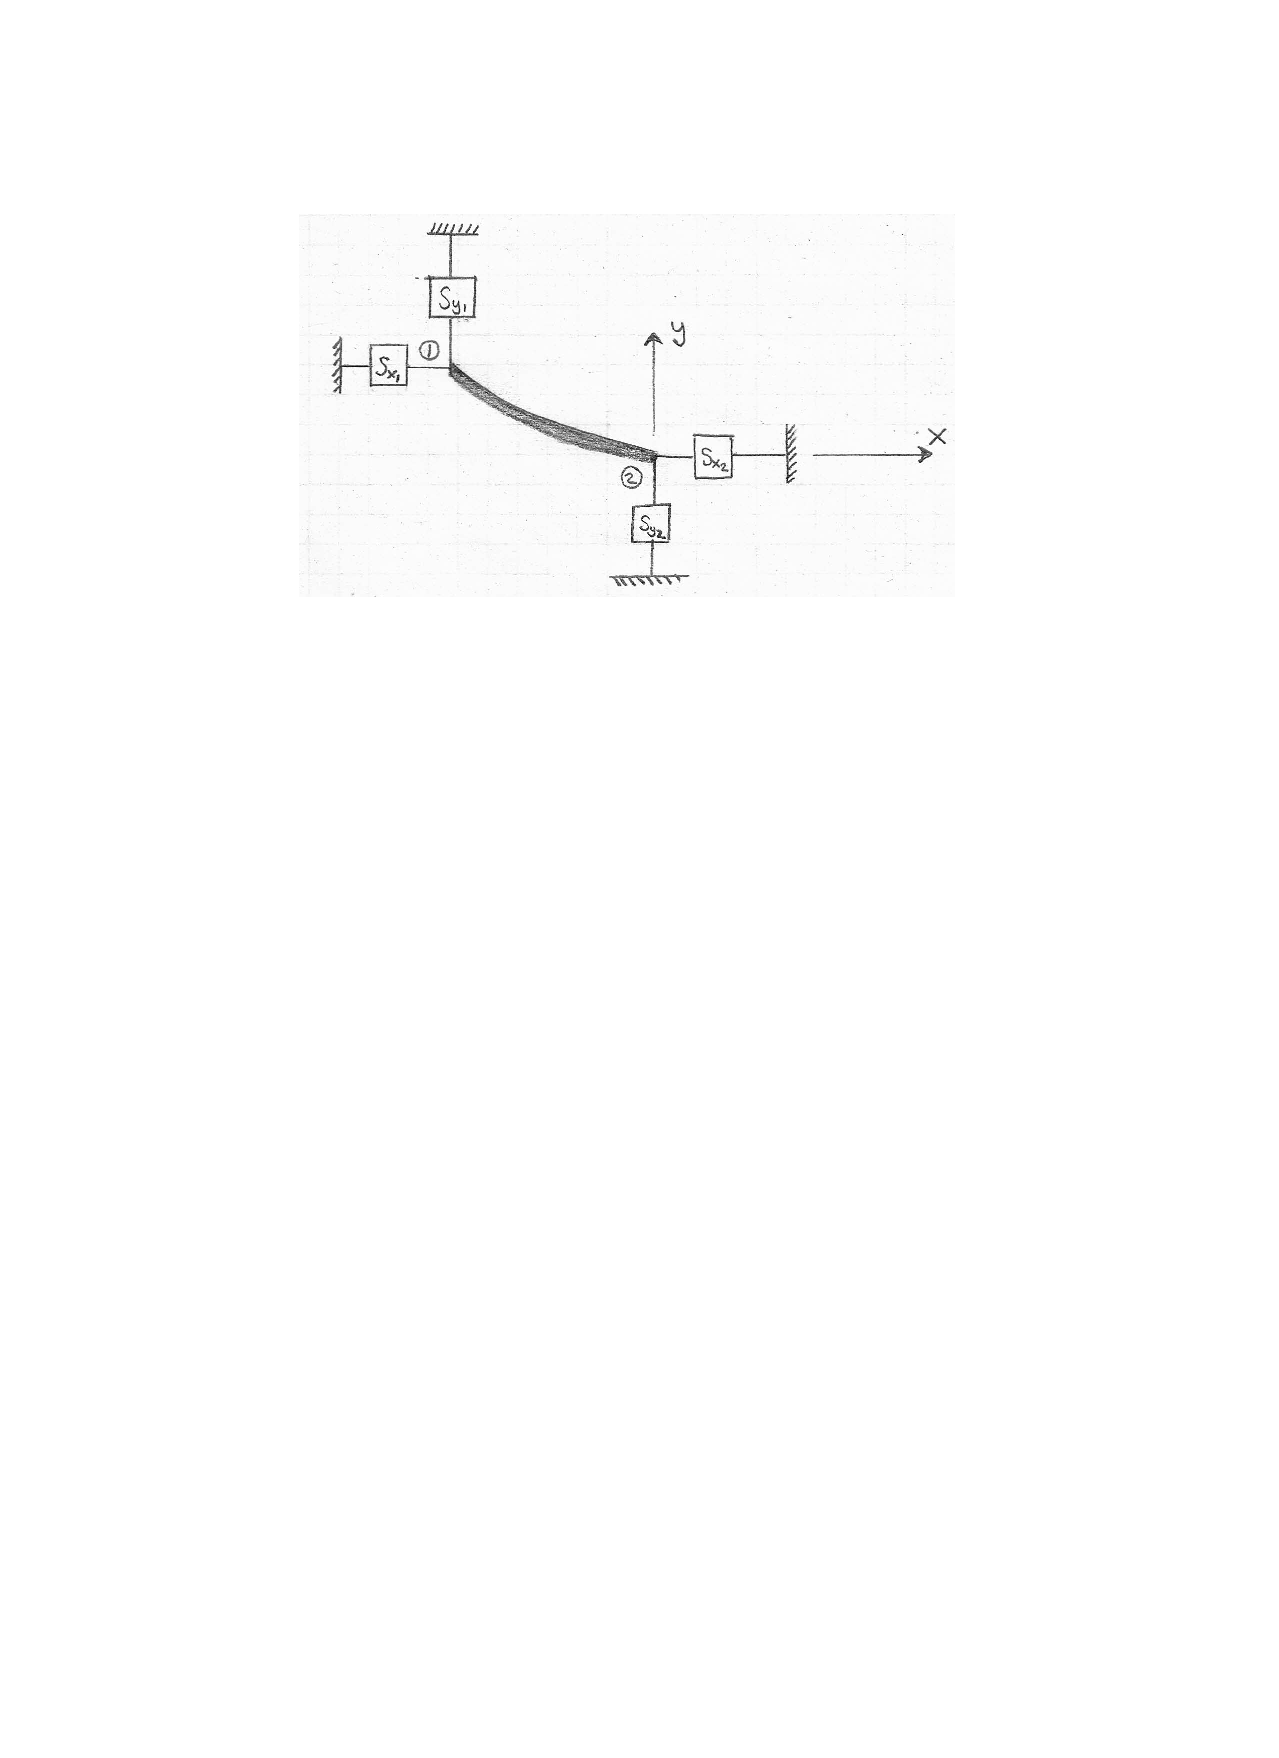
\includegraphics[width=0.75\textwidth]{Figures/Q5_P1_SystemDiagram.pdf}
 \caption{System Diagram}
 \label{sys}
\end{figure}

\begin{figure}	% stiff
 \centering
\begin{tikzpicture}[every node/.style={draw,outer sep=0pt,thick}]
\tikzstyle{spring}=[thick,decorate,decoration={zigzag,pre length=0.3cm,post length=0.3cm,segment length=6}]
\tikzstyle{damper}=[thick,decoration={markings,  
  mark connection node=dmp,
  mark=at position 0.5 with 
  {
    \node (dmp) [thick,inner sep=0pt,transform shape,rotate=-90,minimum width=15pt,minimum height=3pt,draw=none] {};
    \draw [thick] ($(dmp.north east)+(2pt,0)$) -- (dmp.south east) -- (dmp.south west) -- ($(dmp.north west)+(2pt,0)$);
    \draw [thick] ($(dmp.north)+(0,-5pt)$) -- ($(dmp.north)+(0,5pt)$);
  }
}, decorate]

\node (S) [minimum width=2.6cm,minimum height=2.6cm]{};
\node (sw_node) at (S.south) [draw=none,yshift=0cm,xshift=-0.5cm,anchor=north] {};
\node (nw_node) at (S.north) [draw=none,yshift=0.25cm,xshift=-0.5cm,anchor=north] {};
\draw [spring] (sw_node) -- (nw_node);
\node (k_node) at (sw_node) [draw=none,yshift=1.4cm,xshift=-0.4cm,anchor=north] {k};
\node (se_node) at (S.south) [draw=none,yshift=0cm,xshift=0.5cm,anchor=north] {};
\node (ne_node) at (S.north) [draw=none,yshift=0.25cm,xshift=0.5cm,anchor=north] {};
\draw [damper] (se_node) -- (ne_node);
\node (c_node) at (se_node) [draw=none,yshift=1.3cm,xshift=0.4cm,anchor=north] {c};

\end{tikzpicture}
\caption{Stiffener ($S$) Diagram}
\label{stiff}
\end{figure}

\begin{figure}	% rhos
 \centering
 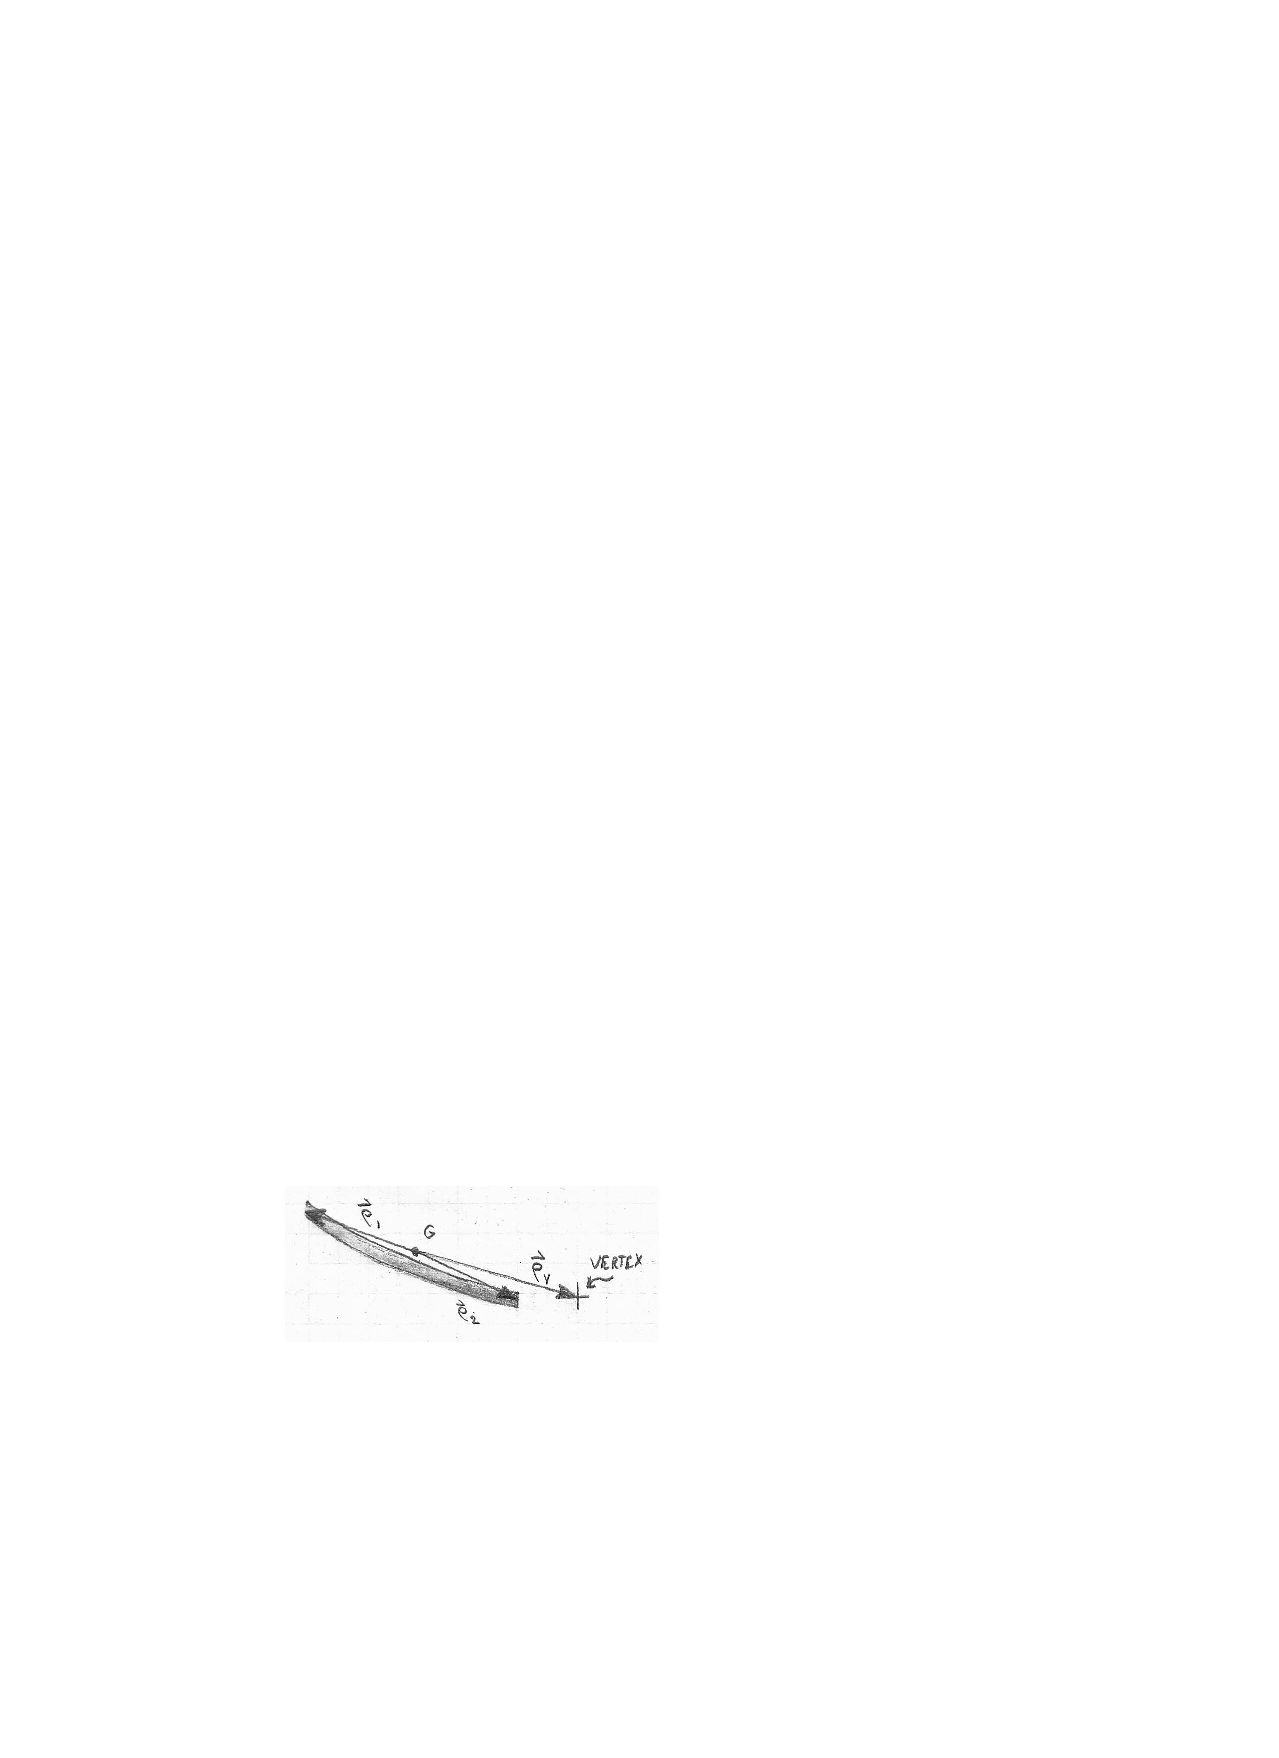
\includegraphics[width=0.5\textwidth]{Figures/Q5_P1_RhoVectors.pdf}
 \caption{CoM and Rho Vectors}
 \label{rhos}
\end{figure}

\begin{figure}		% raytrace
\centering
\begin{tikzpicture}[scale=1.5]
\def\f{4}
\def\xmin{-5} \def\xmax{1}
\def\ymin{0}  \def\ymax{5}
\def\fx{0} \def\fy{\f}
% draw axes
\draw (-.25,-.25) node[auto] {0};
\draw[->,thick] (\xmin,\ymin) -- (\xmax,\ymin) node[right] {$x$};
\draw[->,thick] (\ymin,\ymin) -- (\ymin,\ymax) node[above] {$y$};
% draw off-axis parabolic section
\draw[color=blue,very thick] plot [domain=-4:-2] (\x,{((\x)^2)/(4*\f)});
\draw[color=blue,thick] plot [domain=-4:-2] (\x,{((\x)^2)/(4*\f)-0.1});
\draw[-,color=blue,thick] (-4,{((-4)^2)/(4*\f)-0.1}) -- (-4,{((-4)^2)/(4*\f)});
\draw[-,color=blue,thick] (-2,{((-2)^2)/(4*\f)-0.1}) -- (-2,{((-2)^2)/(4*\f)});
% draw rays
\draw[->,color=red,very thick]  (-4,4) -- (-4,1); \draw[->,color=red,very thick]  (-4,1) -- (\fx,\fy);
\draw[->,color=red,very thick]  (-3,4) -- (-3,0.56); \draw[->,color=red,very thick]  (-3,0.56) -- (\fx,\fy);
\draw[->,color=red,very thick]  (-2,4) -- (-2,0.25); \draw[->,color=red,very thick]  (-2,0.25) -- (\fx,\fy);
\end{tikzpicture}
\caption{Nominal Raytrace}
\label{raytrace}
\end{figure}

 \subsection*{Objective}
 The objective of this analysis is to characterize the evolution of the focal point distribution when subjected to a random disturbance. This is accomplished by Monte Carlo Simulation (MCS) and an example based on user-defined values is presented in the results section. Furthermore, the functional dependence of the output distribution with respect to the input disturbance distribution is observed for a range user-defined values of the input distribution parameters and presented.
 
 % \subsection*{Assumptions}

% \begin{description}
	% \item[1)] The mirror section is an off-axis parabola.
	% \item[2)] All incoming plane waves focus to a single point.
	% \item[3)] The mirror surface is ideal and rigid.
	% \item[4)] The small angle approximation is valid for $\alpha$.
 % \end{description}
\section{Equations of Motion Derivation}

To derive the equations of motion, solve a force-balance for the kinetic equations, then use geometry to develop the kinematic equations and substitute these into the kinetic equations.

\subsection*{Kinetic Equations}

The kinetic equations are formulated by equating the free-body diagram (FBD) with the mass-acceleration diagram as shown in Figure~\ref{FBD=MAD}. The stiffening unit $x$- and $y$-force vector directions are determined by assuming the mirror is displaced in the positive respective direction with positive respective velocity, then inferring the restoring and resistive force imparted by each stiffening unit. The disturbance forces are defined as positive in the $+x$- and $+y$-directions. Referring to the stiffener diagram of Figure~\ref{stiff}, a force-balance for each identical unit as shown in Equation~\eqref{eq:stiffener} characterizes the reactive force at each node.

\begin{equation}
\label{eq:stiffener}
\begin{aligned}
		\sum{F} &= m\ddot{s}\\
		0 &= S - ks - c\dot{s}\\
		S &= ks + c\dot{s}
\end{aligned}
\end{equation}\

\begin{figure}	% FBD=MAD
 \centering
 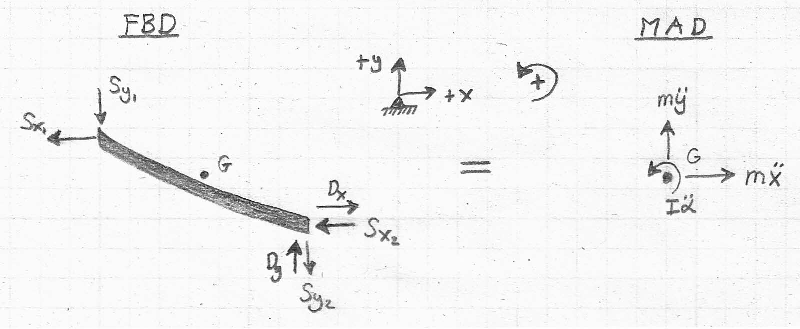
\includegraphics[width=0.75\textwidth]{Figures/Q5_P1_FBD=MAD.pdf}
 \caption{Set the free-body diagram equal to the mass-acceleration diagram to formulate the kinetic equations}
 \label{FBD=MAD}
\end{figure}

\begin{subequations}
\label{eq:kinEQ}
\begin{align}
	\begin{split}
	\sum{F_x} &= m\ddot{x} \\
	m\ddot{x} &= -S_{x_1}-S_{x_2}+Dx \\
	m\ddot{x} &= -kx_1 - c\dot{x_1} - kx_2 - c\dot{x_2} + D_x \\
	\end{split}\\
	\begin{split}
	\sum{F_y} &= m\ddot{y}\\
	m\ddot{y} &= -S_{y_1}-S_{y_2}+Dx \\
	m\ddot{y} &= -ky_1 - c\dot{y_1} - ky_2 - c\dot{y_2} + D_y\\
	\end{split}\\
	\begin{split}
	\sum{M_G} &= I\ddot{\alpha}\\
	I\ddot{\alpha} &= \rho_{2_y}\left[-S_{x_2}+D_x\right] +  \rho_{2_x}\left[-S_{y_2}+D_y\right] + \rho_{y_1}S_{x_1} + \rho_{x_1}S_{y_1}  \\
	I\ddot{\alpha} &= \rho_{2_y}\left[-kx_2 - c\dot{x}_2+D_x\right] +  \rho_{2_x}\left[-ky_2 - c\dot{y}_2+D_y\right] + \rho_{1_y}\left[-kx_1 - c\dot{x}_1\right] + \rho_{1_x}\left[-ky_1 - c\dot{y}_1\right]  \\
	\end{split} \\ \nonumber
\end{align}
\end{subequations}

\subsection*{Kinematic Equations}

The kinematic equations define the interdependencies of the motion of the state variables. For this simulation, these are defined by the geometry of the mechanical system. Specifically, these equations define the positions and velocities of the mirror segment endpoints by the mirror segment CoM position, velocity, and rotation angle.

\begin{equation}
\label{eq:kinemEQ}
\begin{aligned}
		x_1 &= x - d\rho_{1_x} & x_2 &= x + d\rho_{2_x} \\
		\dot{x_1} &= \dot{x} - d\dot{\rho}_{1_x} & \dot{x_2} &= \dot{x} + d\dot{\rho}_{2_x} \\
		y_1 &= y - d\rho_{1_y} & y_2 &= y + d\rho_{2_y} \\
		\dot{y_1} &= \dot{y} - d\dot{\rho}_{1_y} & \dot{y_2} &= \dot{y} + d\dot{\rho}_{2_y}
\end{aligned}
\end{equation}

Where

\begin{equation}
\centering
	\begin{aligned}
	d\rho_{1_x} &= d\rho_1\cos\left( \phi_1 \right) & d\rho_{2_x} &= d\rho_2\cos\left( \phi_2 \right)\\
	d\dot{\rho}_{1_x} &= d\dot{\rho}_1\cos\left( \phi_1 \right) & d\dot{\rho}_{2_x} &= d\dot{\rho}_2\cos\left(\phi_2\right)\\
	d\rho_{1_y} &= d\rho_1\sin\left( \phi_1 \right) & d\rho_{2_y} &= d\rho_2\sin\left( \phi_2 \right)\\
	d\dot{\rho}_{1_y} &= d\dot{\rho}_1\sin\left( \phi_1 \right) & d\dot{\rho}_{2_y} &= d\dot{\rho}_2\sin\left(\phi_2\right)	
	\label{eq:drho}
	\end{aligned}
\end{equation}\

 For this simulation, all rotations about the CoM, $\alpha$, are small enough that the small-angle approximation, Equation~\eqref{eq:smallAngle}, is assumed valid.

\begin{equation}
\centering
	\begin{aligned}
	d\vec{\rho} &\approx \vec{\rho}\sin \left(\alpha\right) &\approx \vec{\rho}\alpha \\
	d\dot{\vec{\rho}} &\approx \vec{\rho} \left[d\left(\sin \left(\alpha\right)\right)\right] &\approx  \vec{\rho}\dot{\alpha}
	\label{eq:smallAngle}
	\end{aligned}
\end{equation}

Such that,

\begin{equation}
\centering
	\begin{aligned}
	d\rho_{1_x} &= \rho_1\alpha\cos\left( \phi_1 \right) & d\rho_{2_x} &= \rho_2\alpha\cos\left( \phi_2 \right)\\
	d\dot{\rho}_{1_x} &= \rho_1\dot{\alpha}\cos\left( \phi_1 \right) & d\dot{\rho}_{2_x} &= \rho_2\dot{\alpha}\cos\left( \phi_2 \right)\\
	d\rho_{1_y} &= \rho_1\alpha\sin\left( \phi_1 \right) & d\rho_{2_y} &= \rho_2\alpha\sin\left( \phi_2 \right)\\
	d\dot{\rho}_{1_y} &= \rho_1\dot{\alpha}\sin\left( \phi_1 \right) & d\dot{\rho}_{2_y} &= \rho_2\dot{\alpha}\sin\left( \phi_2 \right)
	\label{eq:drho}
	\end{aligned}
\end{equation}

The differential changes in position vectors, $d\rho_1$ and $d\rho_2$, are illustrated by Figures~\ref{drho12}.

\begin{figure}	% drho12
 \centering
 \subfigure[]{
 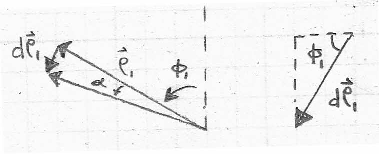
\includegraphics[width=0.6\textwidth]{Figures/Q5_P1_Rho1.pdf}}
 \subfigure[]{
 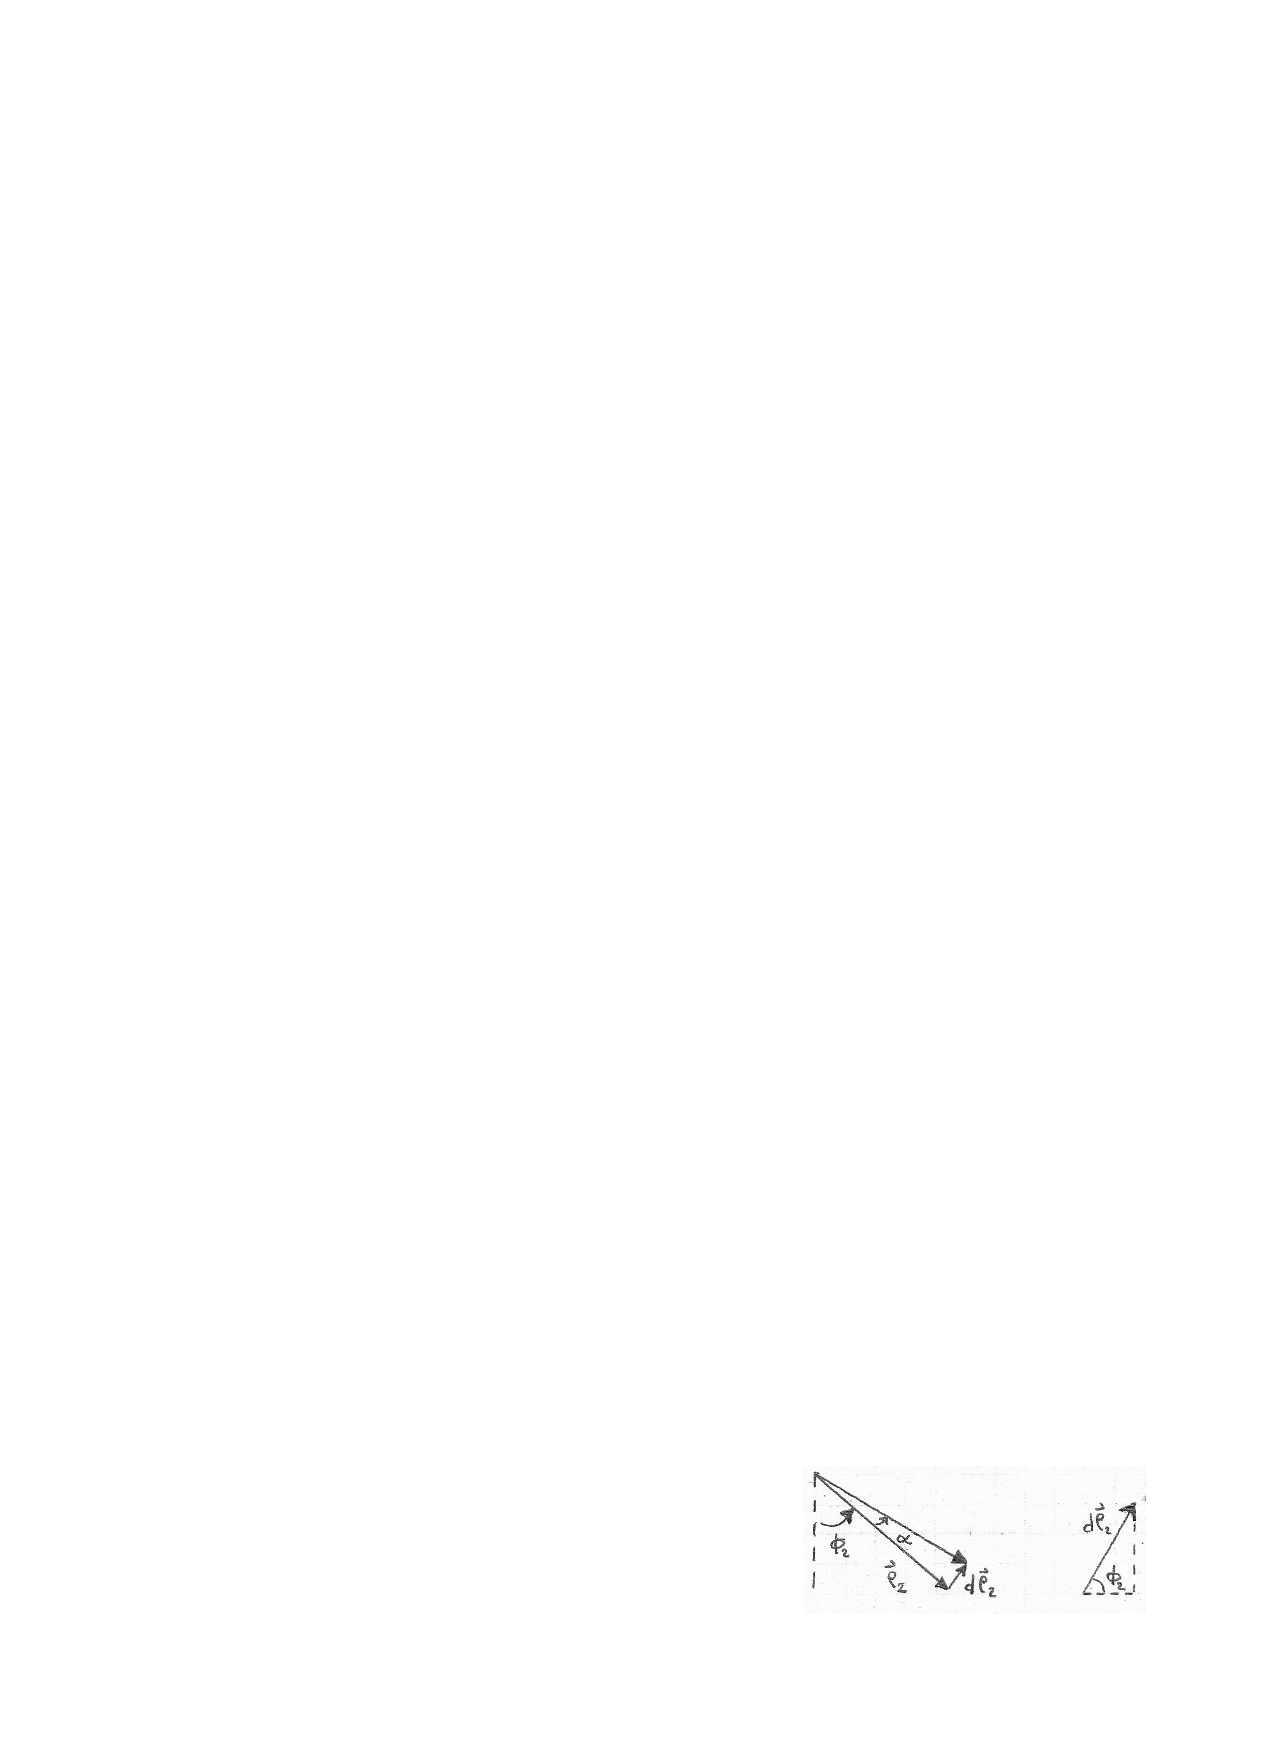
\includegraphics[width=0.5\textwidth]{Figures/Q5_P1_Rho2.pdf}}
 \caption{Rho Vectors}
 \label{drho12}
\end{figure}

\subsection*{Centroid Location}

Working with an off-axis parabolic mirror segment requires intermediate calculations to find the location of the centroid with respect to the vertex. The simulation presented assumes the $x$-coordinate of both mirror endpoints is known. First, calculate the arc length, $L$, of the mirror as follows.

\begin{equation}
\label{eq:arclength}
\centering
\begin{aligned}
	(dL)^2 &= (dx)^2 + (dy)^2 \\
	\frac{dL}{dx} &= \sqrt{1+\left(\frac{dy}{dx}\right)^2} \\
	L &= \bigintss_a^b \sqrt{1+\left(\frac{dy}{dx}\right)^2}dx
\end{aligned}
\end{equation}\

Then, find the mass of the mirror using a constant length density, $\rho_L$, and the arc length, $L$, between the known endpoint locations, $x_1$ and $x_2$.

\begin{equation}
\label{eq:mass}
\centering
\begin{aligned}
	m &= \rho_L L \\
	&= \rho_L \bigintss_{x_1}^{x_2} \sqrt{1+\left(\frac{dy}{dx}\right)^2}dx
\end{aligned}
\end{equation}\

Next, calculate the moments about the $x$- and $y$-axes. The moment is the mass of a differential element multiplied by the perpendicular distance from the axis.

\begin{equation}
\label{eq:moment1}
\centering
\begin{aligned}
	M_x &= \rho_L \bigintss_{x_1}^{x_2} y(x)\sqrt{1+\left(\frac{dy}{dx}\right)^2}dx \\
	M_y &= \rho_L \bigintss_{x_1}^{x_2} x\sqrt{1+\left(\frac{dy}{dx}\right)^2}dx
\end{aligned}
\end{equation}\

To calculate the centroid location, note that the moment about an axis is equal to the mass located at the centroid.\\

\begin{equation}
\label{eq:moment2}
\centering
\begin{aligned}
	M_x &= m\bar{y} \\
	M_y &= m\bar{x}
\end{aligned}
\end{equation}\

Thus,

\begin{equation}
\label{eq:centroid}
\centering
\begin{aligned}
	\bar{x} &= \frac{M_y}{m} \\
	&= \frac{\rho_L}{m} \bigintss_{x_1}^{x_2} x\sqrt{1+\left(\frac{dy}{dx}\right)^2}dx \\
	\\
	\bar{y} &= \frac{M_x}{m} \\
	&= \frac{\rho_L}{m} \bigintss_{x_1}^{x_2} y(x)\sqrt{1+\left(\frac{dy}{dx}\right)^2}dx
\end{aligned}
\end{equation}\

For a parabola,

\begin{equation}
\label{parabola}
\centering
\begin{aligned}
	y(x) &= \frac{1}{4f}x^2 \\
	\\
	\frac{dy}{dx} &= \frac{1}{2f}x
\end{aligned}
\end{equation}\\

$\vec{\rho}_V$, $\vec{\rho}_1$, and $\vec{\rho}_2$ of Figure~\ref{drho12} are easily calculated as the difference between the associated point position vectors.

\subsection*{Equations of Motion}

Substitute Equations~\eqref{eq:drho} into~\eqref{eq:kinemEQ}, then \eqref{eq:kinemEQ} into \eqref{eq:kinEQ} to generate equations of motion with $x$ and $y$ position of the CoM and $\alpha$ as the system states.

\begin{subequations}
\label{eq:fullEoM}
\centering
\begin{align}
	\ddot{x} &= \frac{1}{m}\left[-k\left(x - d\rho_{1_x}\right) -c\left(\dot{x} - d\dot{\rho}_{1_x}\right) - k\left(x - d\rho_{2_x}\right) -c\left(\dot{x} - d\dot{\rho}_{2_x}\right) + D_x \right]\\
	\nonumber \\
	\ddot{y} &= \frac{1}{m}\left[-k\left(y - d\rho_{1_y}\right) -c\left(\dot{y} - d\dot{\rho}_{1_y}\right) - k\left(y - d\rho_{2_y}\right) -c\left(\dot{y} - d\dot{\rho}_{2_y}\right) + D_y \right] \\
	\nonumber \\
	\begin{split}
	\ddot{\alpha} &= \frac{1}{I} \Biggl\{ \rho_{2_y}\left[-k\left(x - d\rho_{2_x}\right) - c\left(\dot{x} - d\dot{\rho}_{2_x}\right)+D_x\right] +  
													 \rho_{2_x}\left[-k\left(y - d\rho_{2_y}\right) - c\left(\dot{y} - d\dot{\rho}_{2_y}\right)+D_y\right]  \\
						&					  + \rho_{y_1}\left[-k\left(x - d\rho_{1_x}\right) - c\left(\dot{x} - d\dot{\rho}_{1_x}\right)\right] + 
													 \rho_{x_1}\left[-k\left(y - d\rho_{1_y}\right)  - c\left(\dot{y} - d\dot{\rho}_{1_y}\right)\right]  \Biggr\}
	\end{split}
\end{align}
\end{subequations}

\section{Simulation}

To simulate the dynamics of the mirror response, use MATLAB and generate random input disturbance vectors. The random disturbance, $\vec{D}$, is applied at the node \#2 (right) and given as Equation~\eqref{eq:dist}. The disturbance input is a force with random magnitude, $r$, and random direction, $\theta$, where $r \sim \mathcal{N}\left(r_0,\sigma_0\right)$ and $\theta \sim \mathcal{U}\left(0,2\pi\right)$. For this simulation, the input is an impulse at $t=0$, so the only non-zero value in the disturbance vector is at the initial state.\\

\begin{equation}
\label{eq:dist}
	\vec{D} = \left[
					\begin{array}{c}
					D_x\\
					D_y\\
					\end{array}
					\right]
				= \left[
					\begin{array}{c}
					r\cos{\theta}\\
					r\sin{\theta}\\
					\end{array}
					\right]
\end{equation}\\

 A first-order state-space representation of the equations of motion is integrated using \texttt{ODE45()} in MATLAB. Thus, for a realization of the random disturbance, a numerical deterministic solution of the mirror dynamics is obtained. The output is chosen to be the optical performance parameter of maximum spot size radius based on an exact raytrace. At each state, an exact raytrace as shown in a perturbed case by Figure~\ref{rt} is simulated in MATLAB using objects of \texttt{MirrorClass.m} and \texttt{RayClass.m}. In the focal plane, Figure~\ref{sd}, the maximum spot size radius is calculated as the euclidean norm of the chief ray intersection point with the intersection point of the ray farthest from the chief ray in the focal plane. The deviation of the chief ray intersection point from its nominal location is not considered. \\
 
 \begin{figure}	% rtsd
 \centering
 \subfigure[]{
 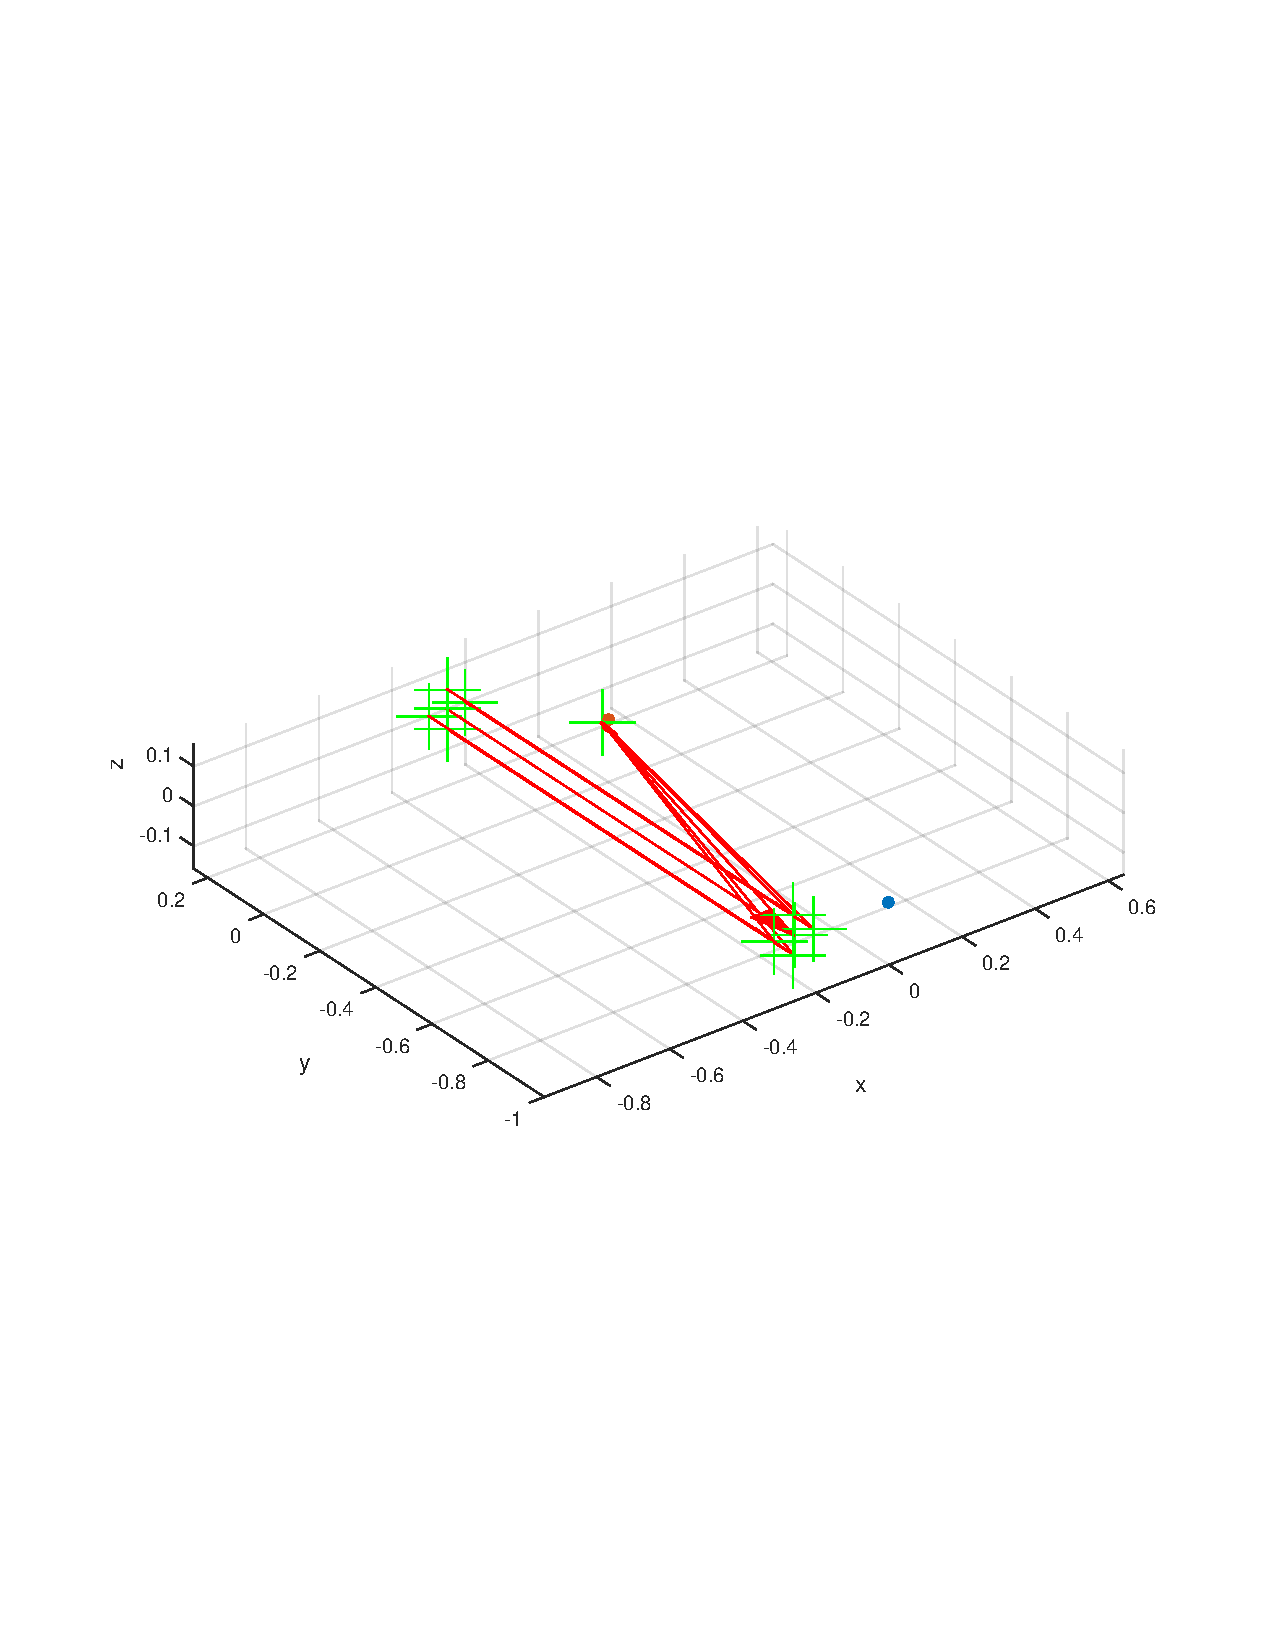
\includegraphics[width=0.45\textwidth,trim=1cm 6cm 2cm 6cm,clip]{Figures/Q5P1_raytrace.pdf}
 \label{rt}}
 \subfigure[]{
 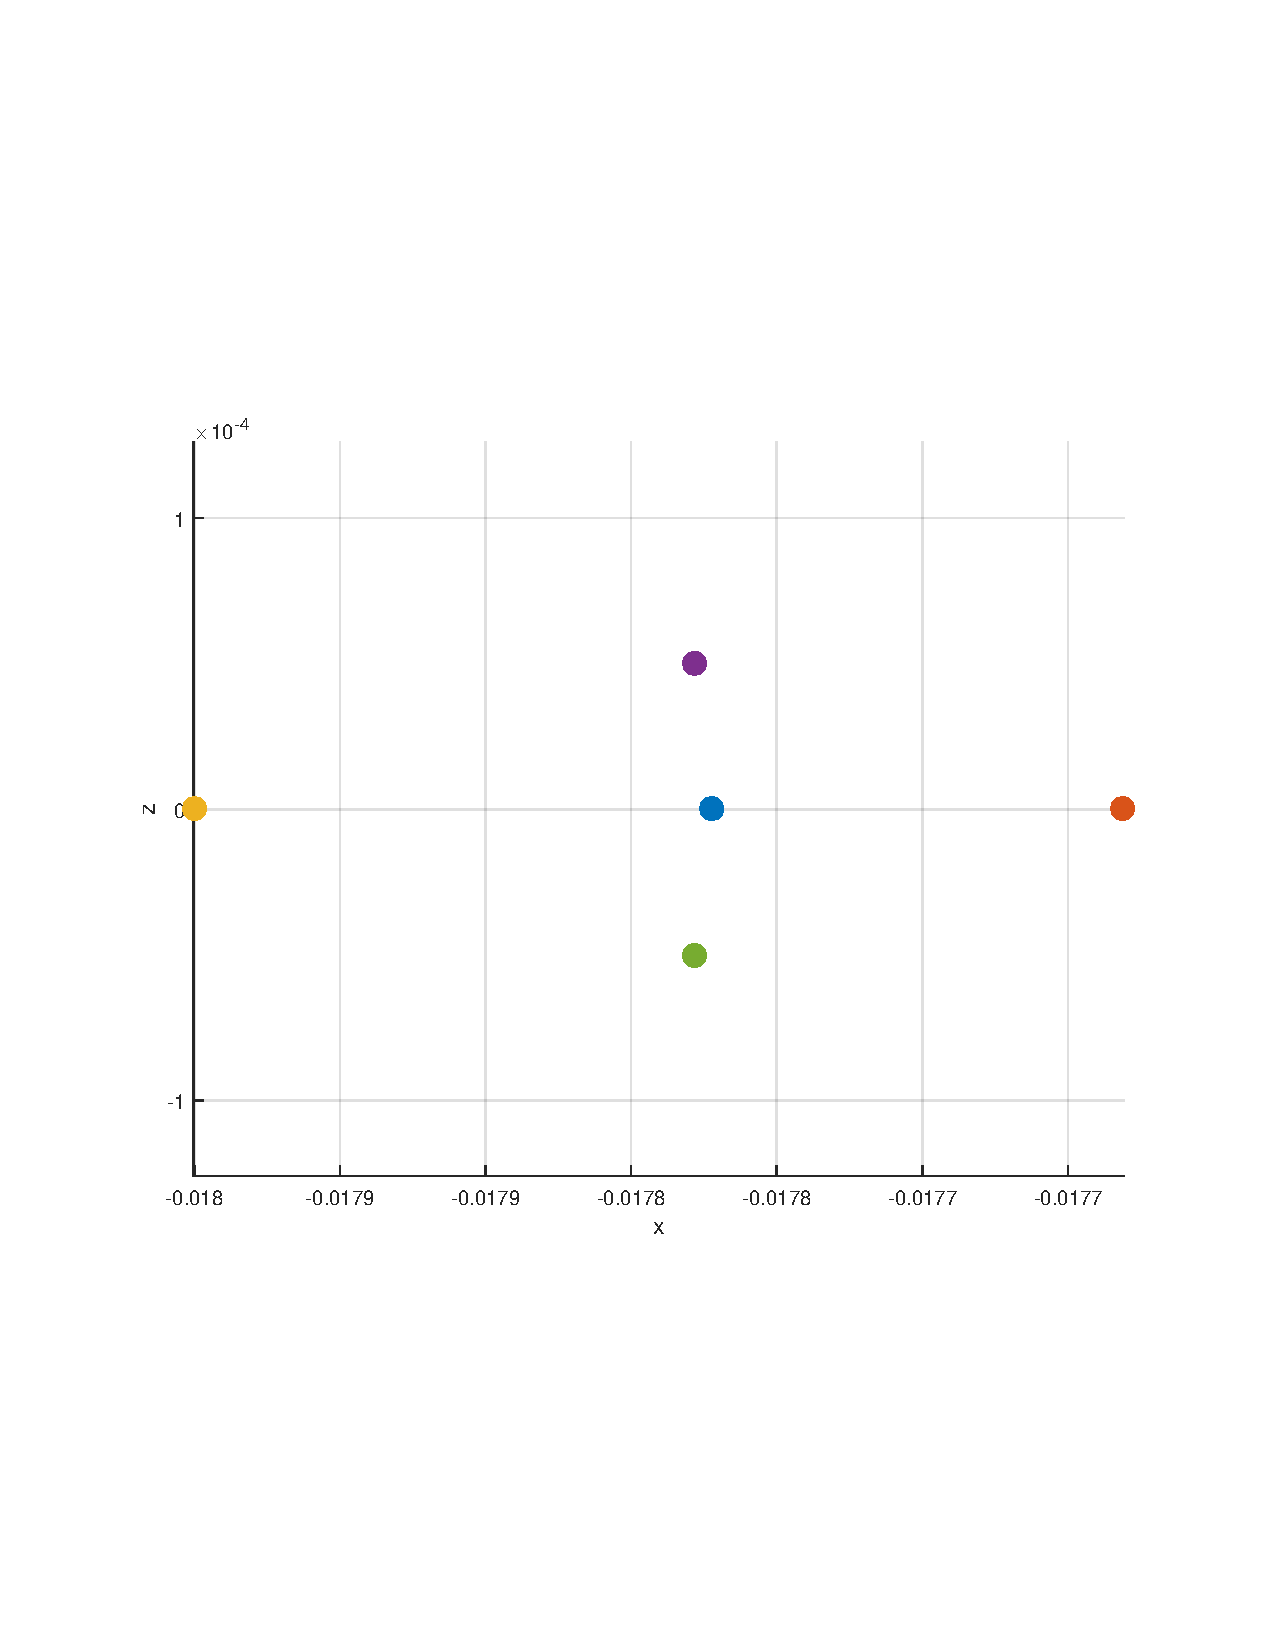
\includegraphics[width=0.45\textwidth,trim=1cm 6cm 2cm 6cm,clip]{Figures/Q5P1_spotdiagram.pdf}
 \label{sd}}
 \caption{Raytrace (a) and corresponding detector plane spot diagram (b) for mirror in a perturbed state (rotation about the z-axis).}
 \label{rtsd}
\end{figure}
 
 When a Monte Carlo Simulation is run, a complete state history of the input and output are available for each realization and each combination of disturbance distribution parameters, $r_0$ and $\sigma_0$. The cost functional of each realization is the average of the maximum spot size radius at each state. A Gaussian distribution is assumed for the scalar output performance measure and the mean and standard deviation of this average are calculated for all realizations of a given distribution (i.e.\ $r_{ss_{max}} \sim \mathcal{N}\left(\mu_{out},\sigma_{out}\right)$ given $r_0$ and $\theta_0$). Thus, the output distribution parameters, $\mu_{out}$ and $\sigma_{out}$, are generated as a function of the input disturbance distribution parameters, $r_0$ and $\theta_0$.\\
 
 \subsection*{MATLAB Simulation Details}

\begin{sloppypar} 
The MATLAB simulation script first defines the geometric properties of the system. The function, \texttt{calcConicCentroid.m}, returns the indices of the centroid, point 1, and point 2 as well as the mass and moment of inertia of the parabolic mirror segment. Next, values are assigned to the spring rate and damping coefficient and the simulation time is specified. The MCS is accomplished by generating sample realizations of the disturbances, simulating mirror dynamics, and calculating the corresponding optical outputs a number of times for each disturbance distribution. Function \texttt{Q5\_Realization.m} returns the output dynamics and the spotsize for a given $r_0$ and $\sigma_0$, then the mean and standard deviation is computed for each combination. \\
 \end{sloppypar}
 
The function \texttt{Q5\_Realization.m} generates the random impulse disturbance based on the supplied distribution parameters. Function \texttt{state\_eqns.m} is supplied the time span, initial guess, and disturbance vector and the deterministic solution is computed by numerical integration of the first-order state equations using \texttt{ODE45.m}.From the output state vector, the mirror vertex position is calculated. The change in vertex position from the nominal location as well as the perturbed angle is passed to function \texttt{SingleMirror\_SpotSize.m}.\\
 
\texttt{SingleMirror\_SpotSize.m} defines properties of the mirror conic section and the direction of the input beam. Mirror objects are constructed from \texttt{MirrorClass.m} with the mirror properties and these mirror objects are used to construct ray objects from \texttt{RayClass.m}. Each ray object can be thought of as one complete trace of a ray through the optical system. It contains a segment for each propagation step and the coordinates of each endpoint of each segment. The class files \texttt{MirrorClass.m} and \texttt{RayClass.m} utilize and compliment work presented by Breckenridge and Redding.~\cite{RedBreck} The final surface in the raytrace is the reference surface and the intersection point of the rays with that plane defines the spot diagram. \texttt{SingleMirror\_SpotSize.m} finishes by calculating the distance between the chief ray and each of the marginal ray reference surface intersection points and determines the maximum distance. This maximum distance is defined as the spot size for this analysis.After all realizations have run and the distribution of the output has been calculated, the results are plotted.

 \section{Results}

The resulting motion caused by one realization of the input disturbance is plotted in Figure~\ref{motionPlots}. It can be seen the disturbance is an impulse and the resulting motion is stable, settling back to the equilibrium point. Figure~\ref{ssEvolution} depicts the evolution of the maximum radius of the spot size during the simulation. The spot size radius is a positive definite quantity and the average spot size over the simulation time is the output metric.\\

\begin{figure}
	\centering
	\subfigure[]{
	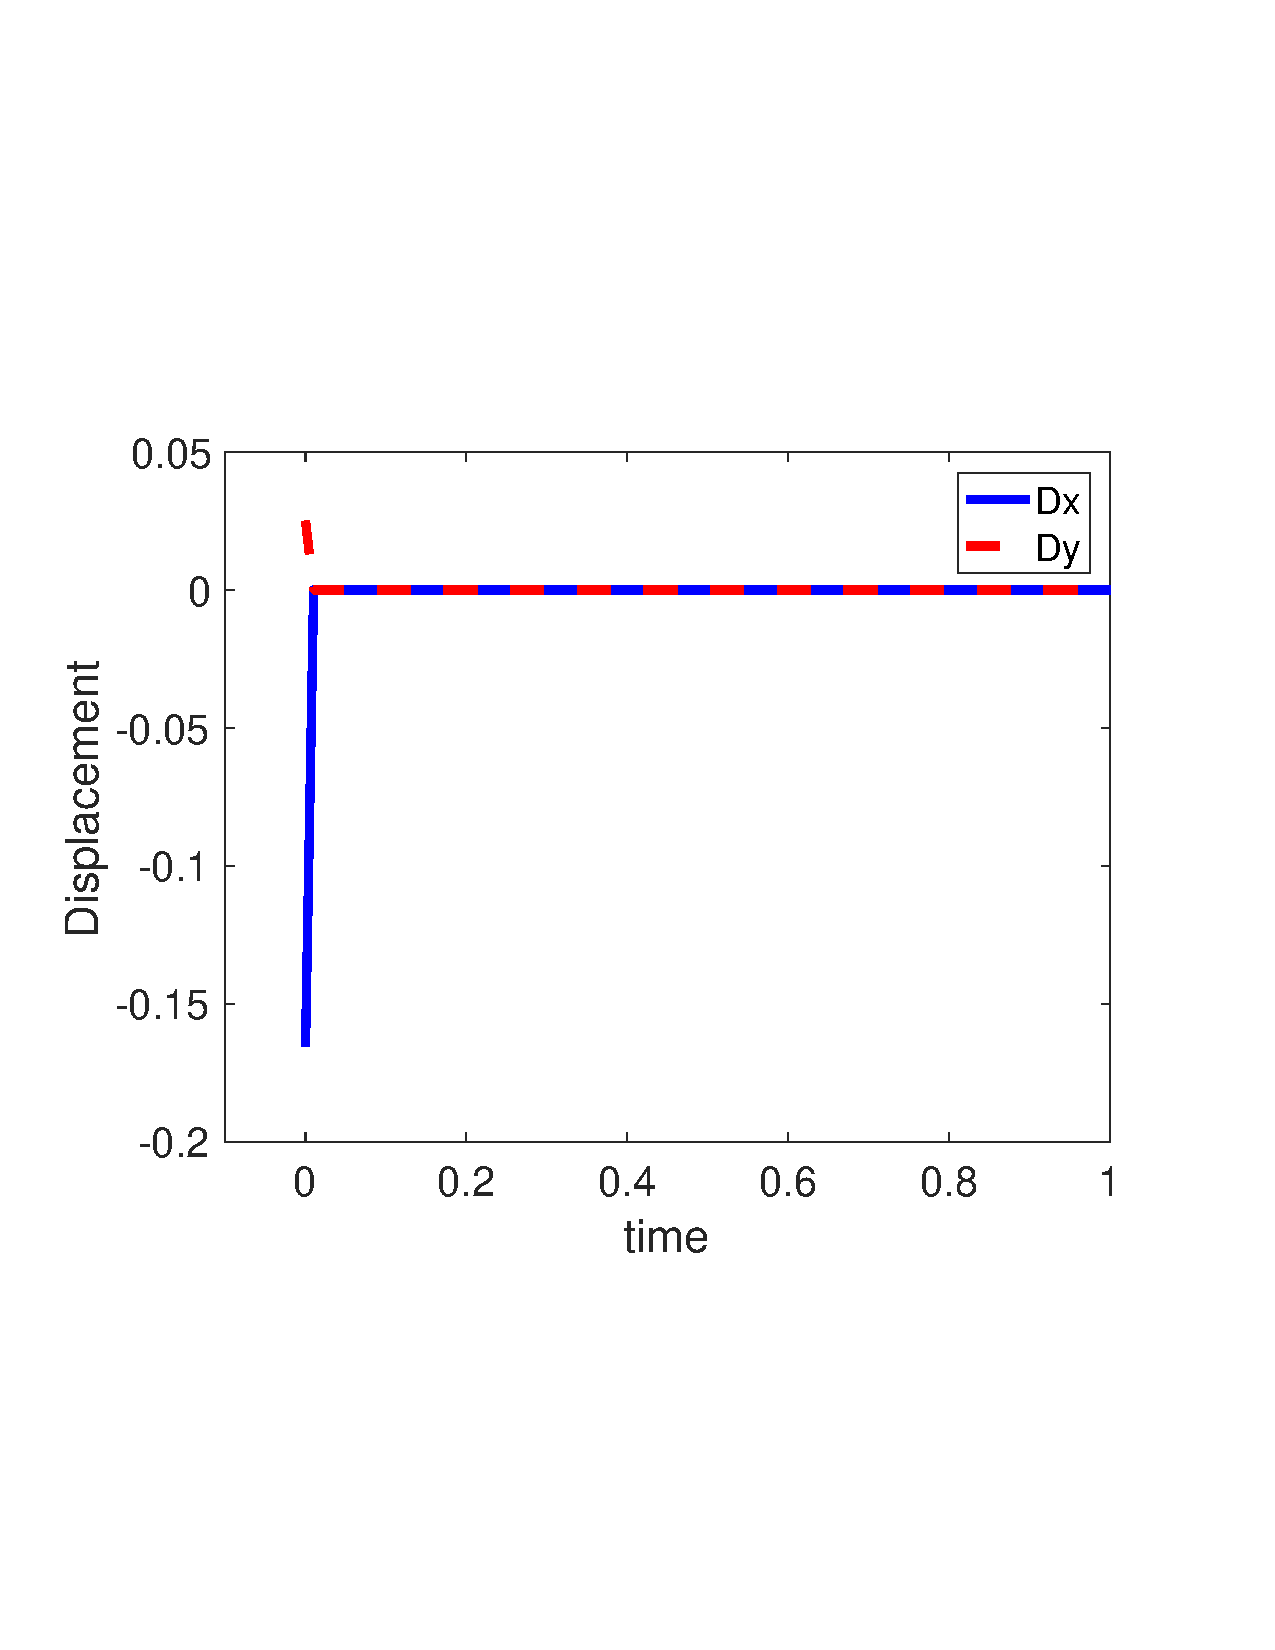
\includegraphics[width=0.45\textwidth,trim=0.8cm 6cm 2cm 6cm,clip]{Figures/Q5P1_real_Disturbance.pdf}}
	\subfigure[]{
	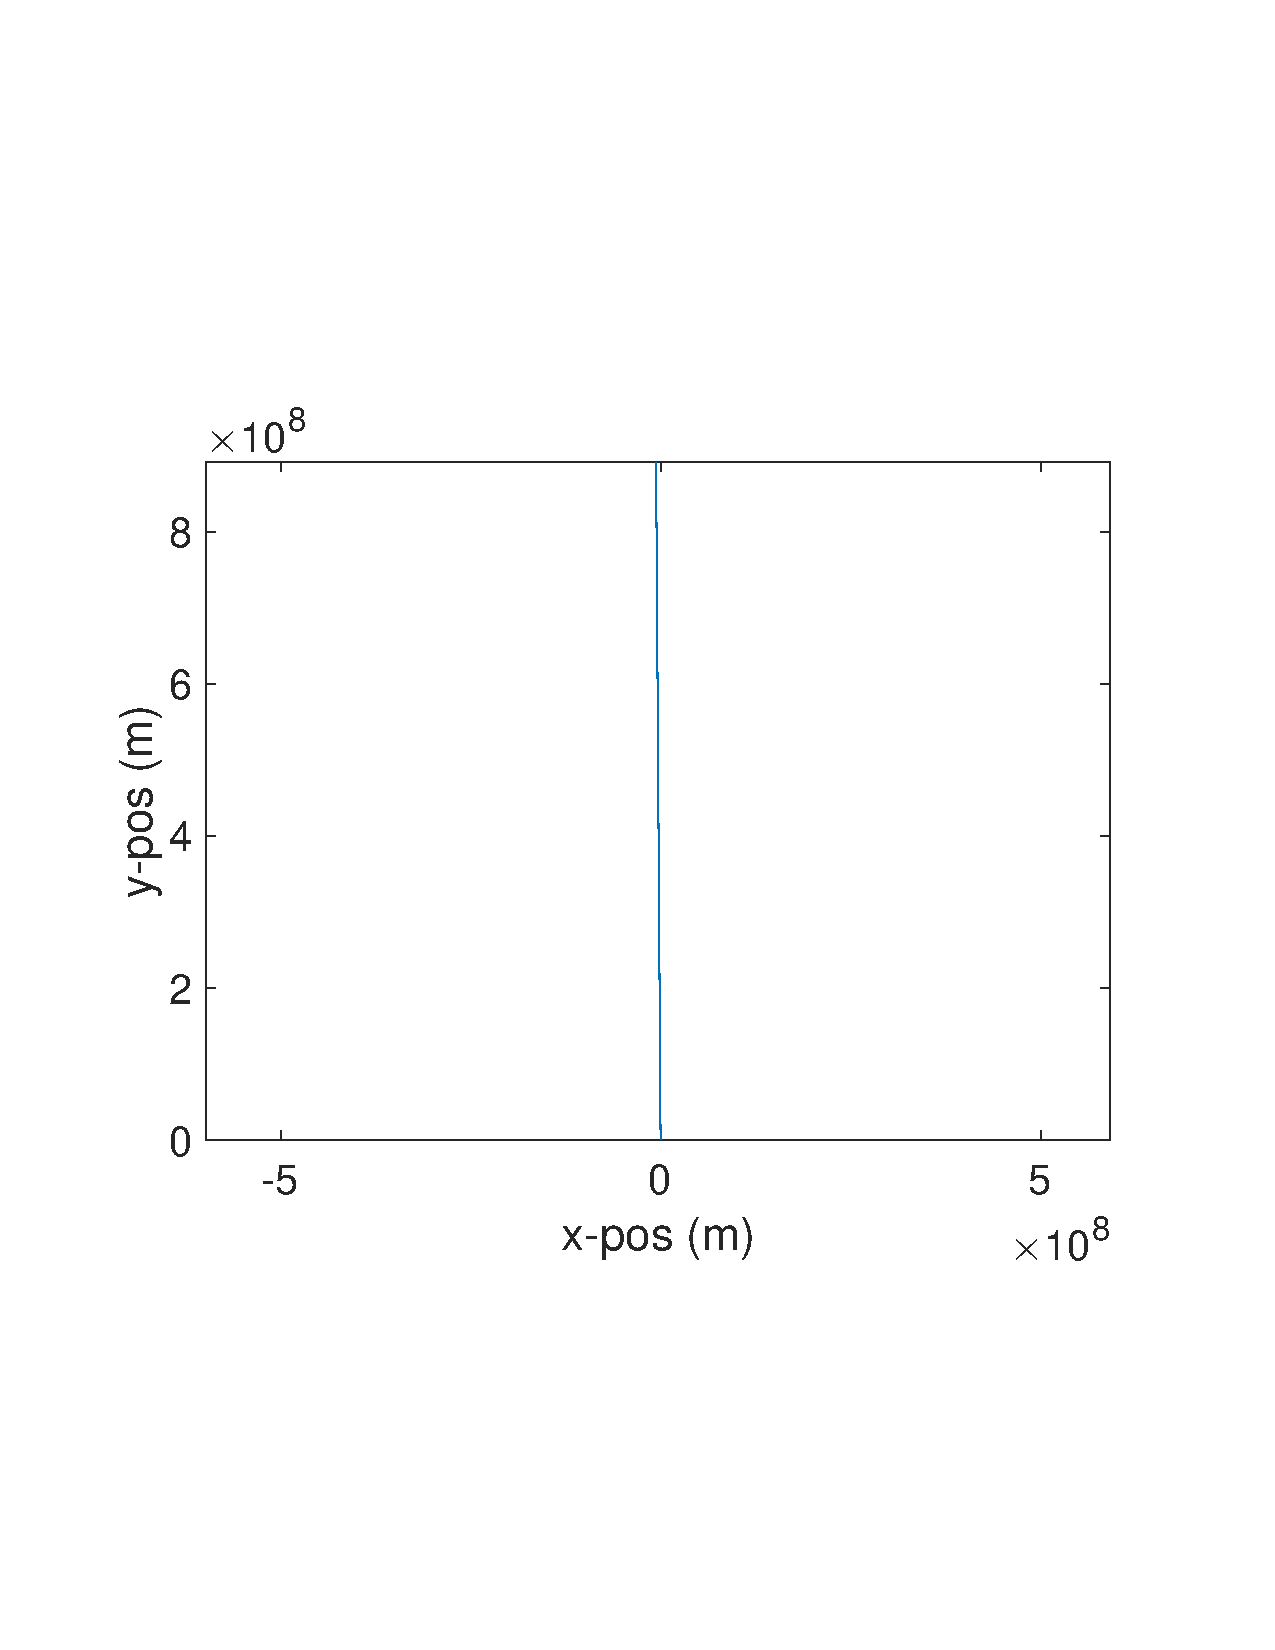
\includegraphics[width=0.45\textwidth,trim=0.8cm 6cm 2cm 6cm,clip]{Figures/Q5P1_real_CoM_Motion.pdf}}
	\subfigure[]{
	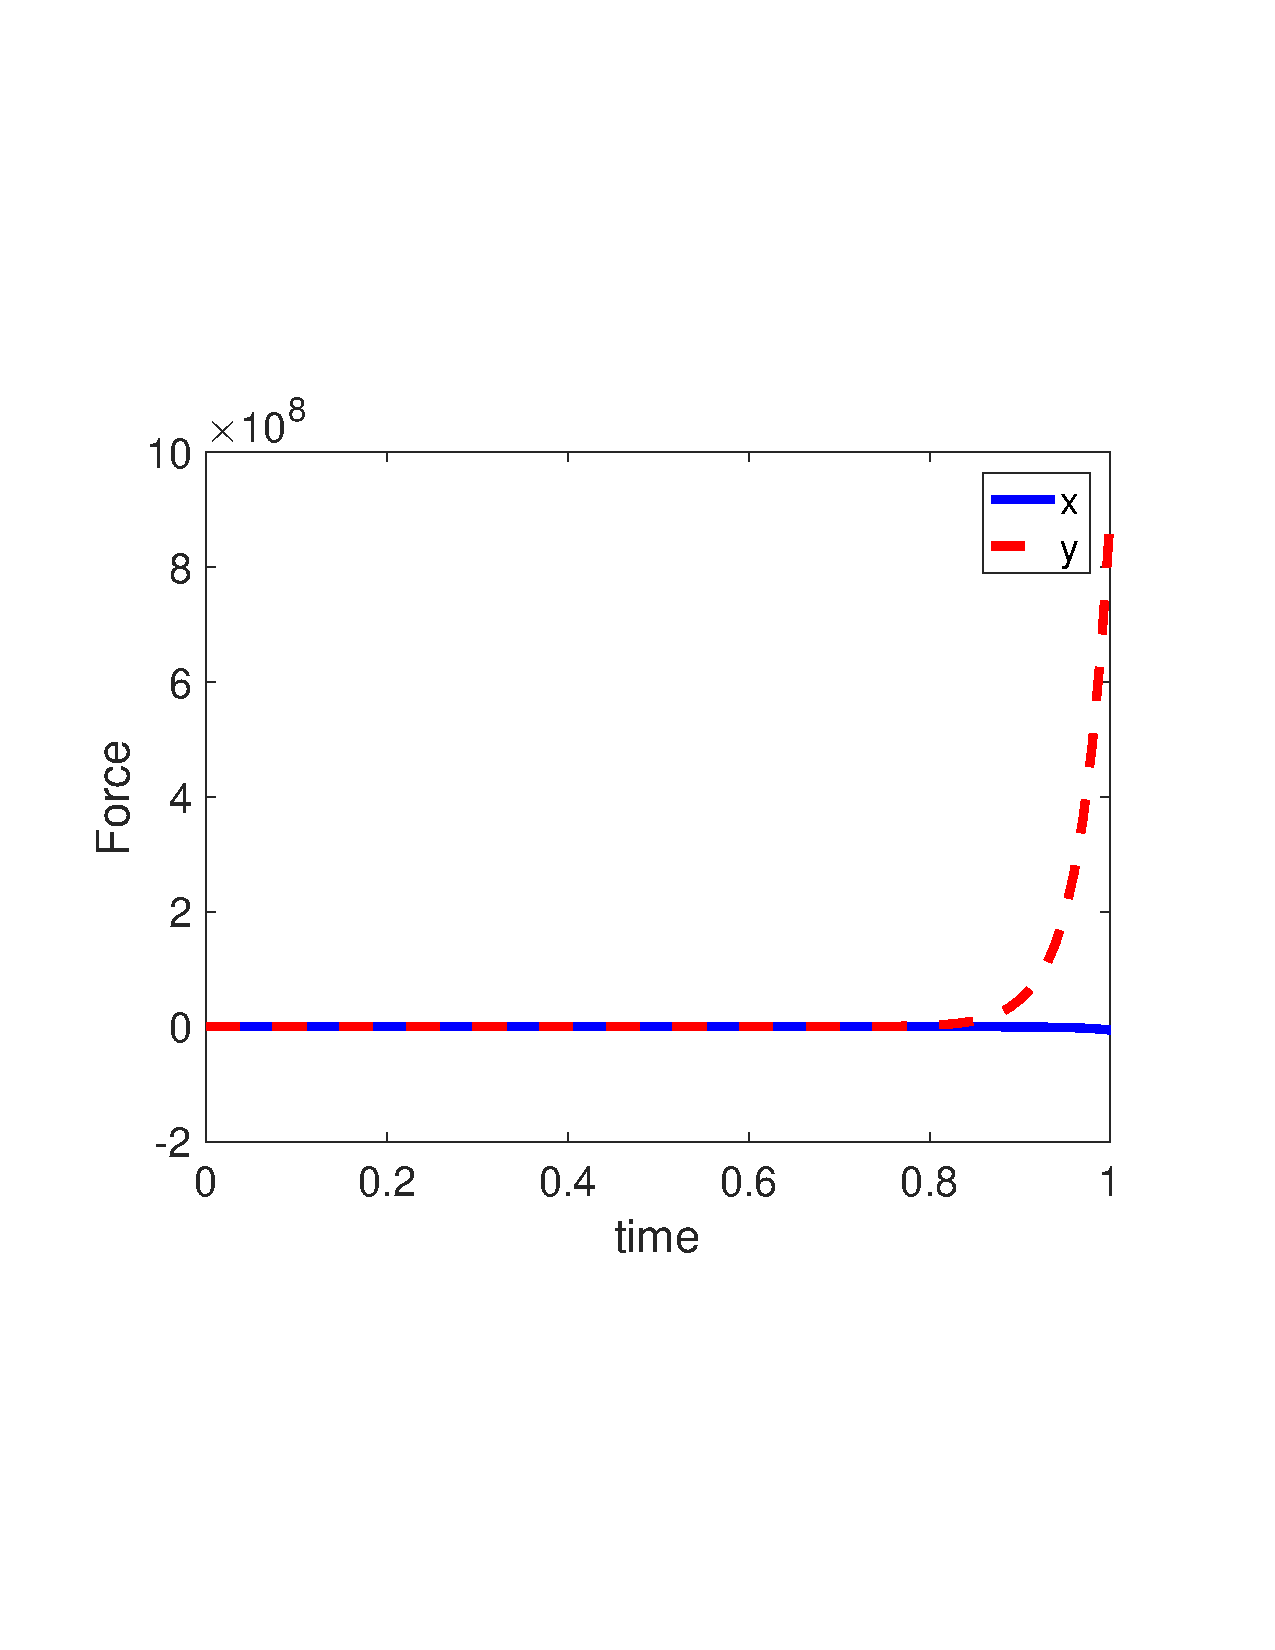
\includegraphics[width=0.45\textwidth,trim=0.8cm 6cm 2cm 6cm,clip]{Figures/Q5P1_real_CoM_LinDisp.pdf}}
	\subfigure[]{
	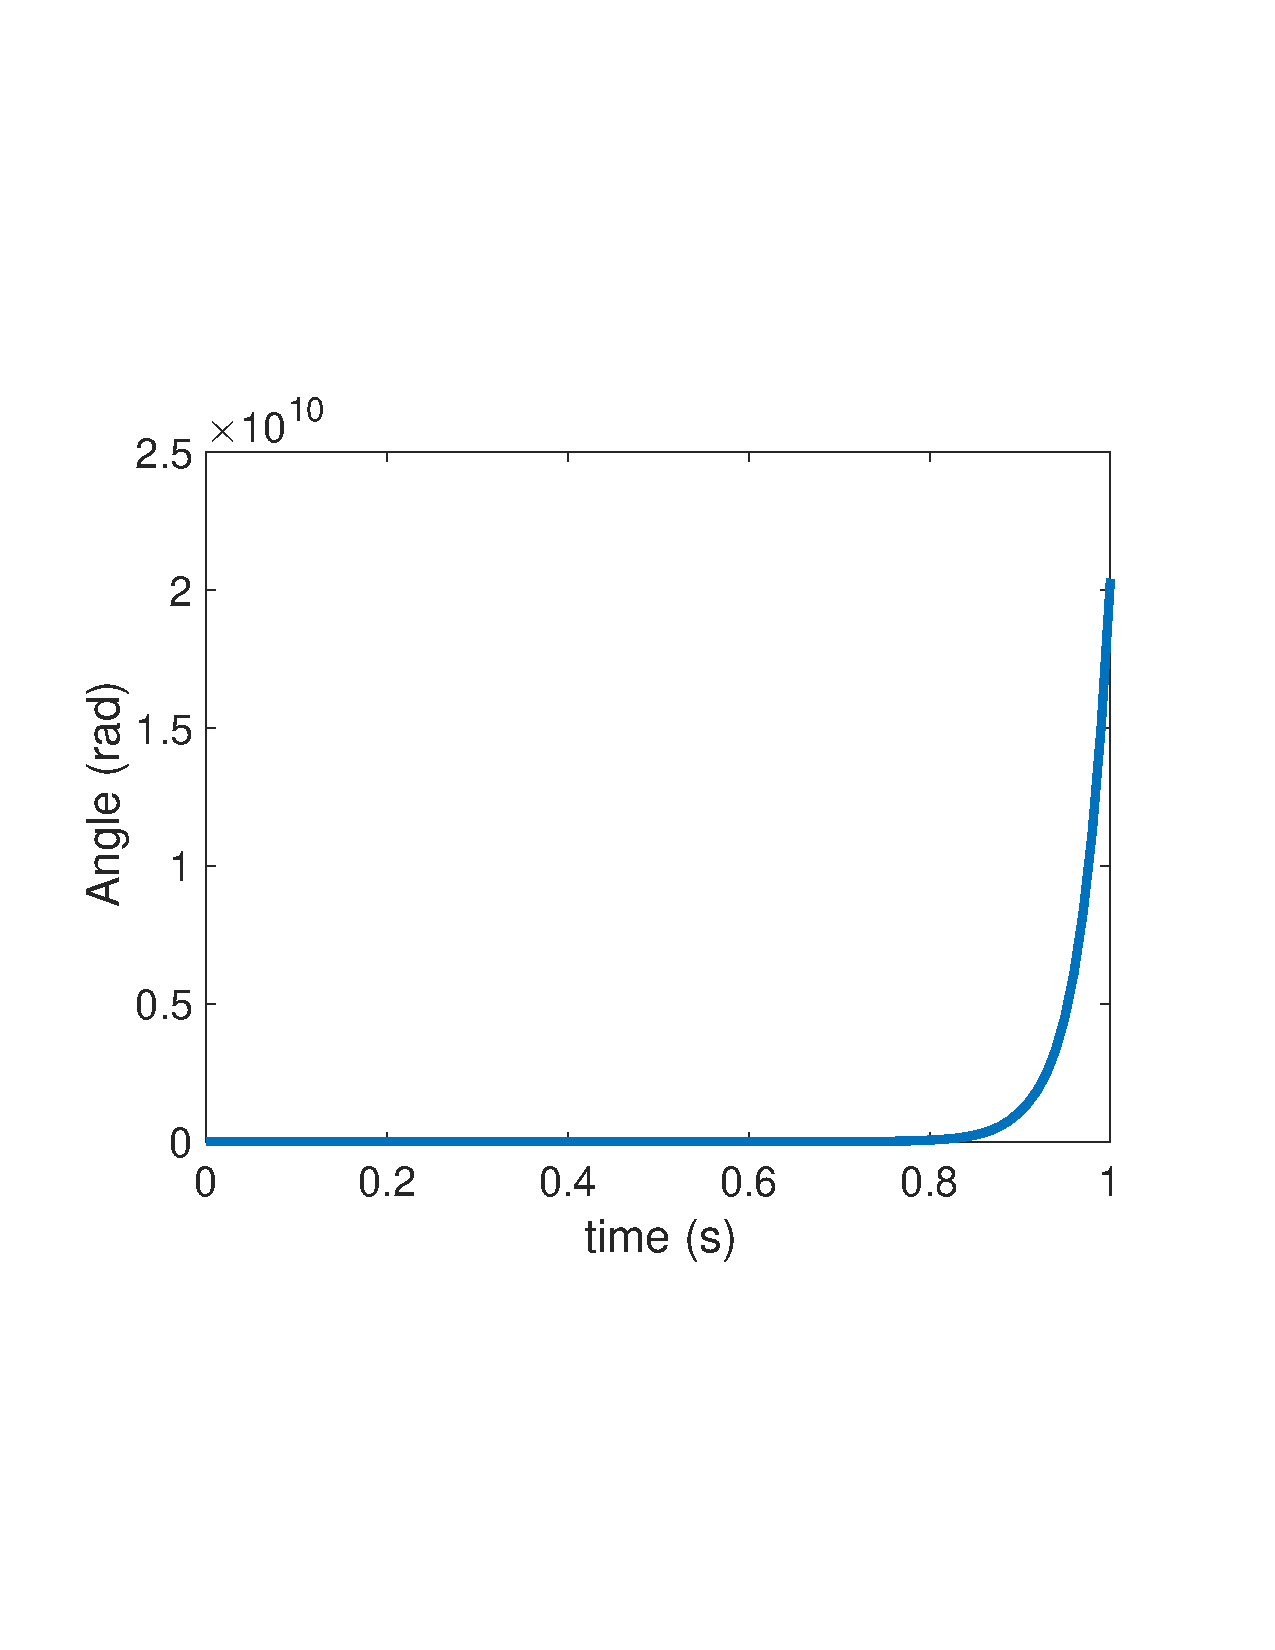
\includegraphics[width=0.45\textwidth,trim=0.8cm 6cm 2cm 6cm,clip]{Figures/Q5P1_real_CoM_AngDisp.pdf}}
	\caption{Dynamic responses to force disturbance. (a) Impulse force disturbance input at node \#2. (b) CoM motion. (c) CoM linear displacements. (d) Mirror angular displacement.}
	\label{motionPlots}
\end{figure}

\begin{figure}
	\centering
	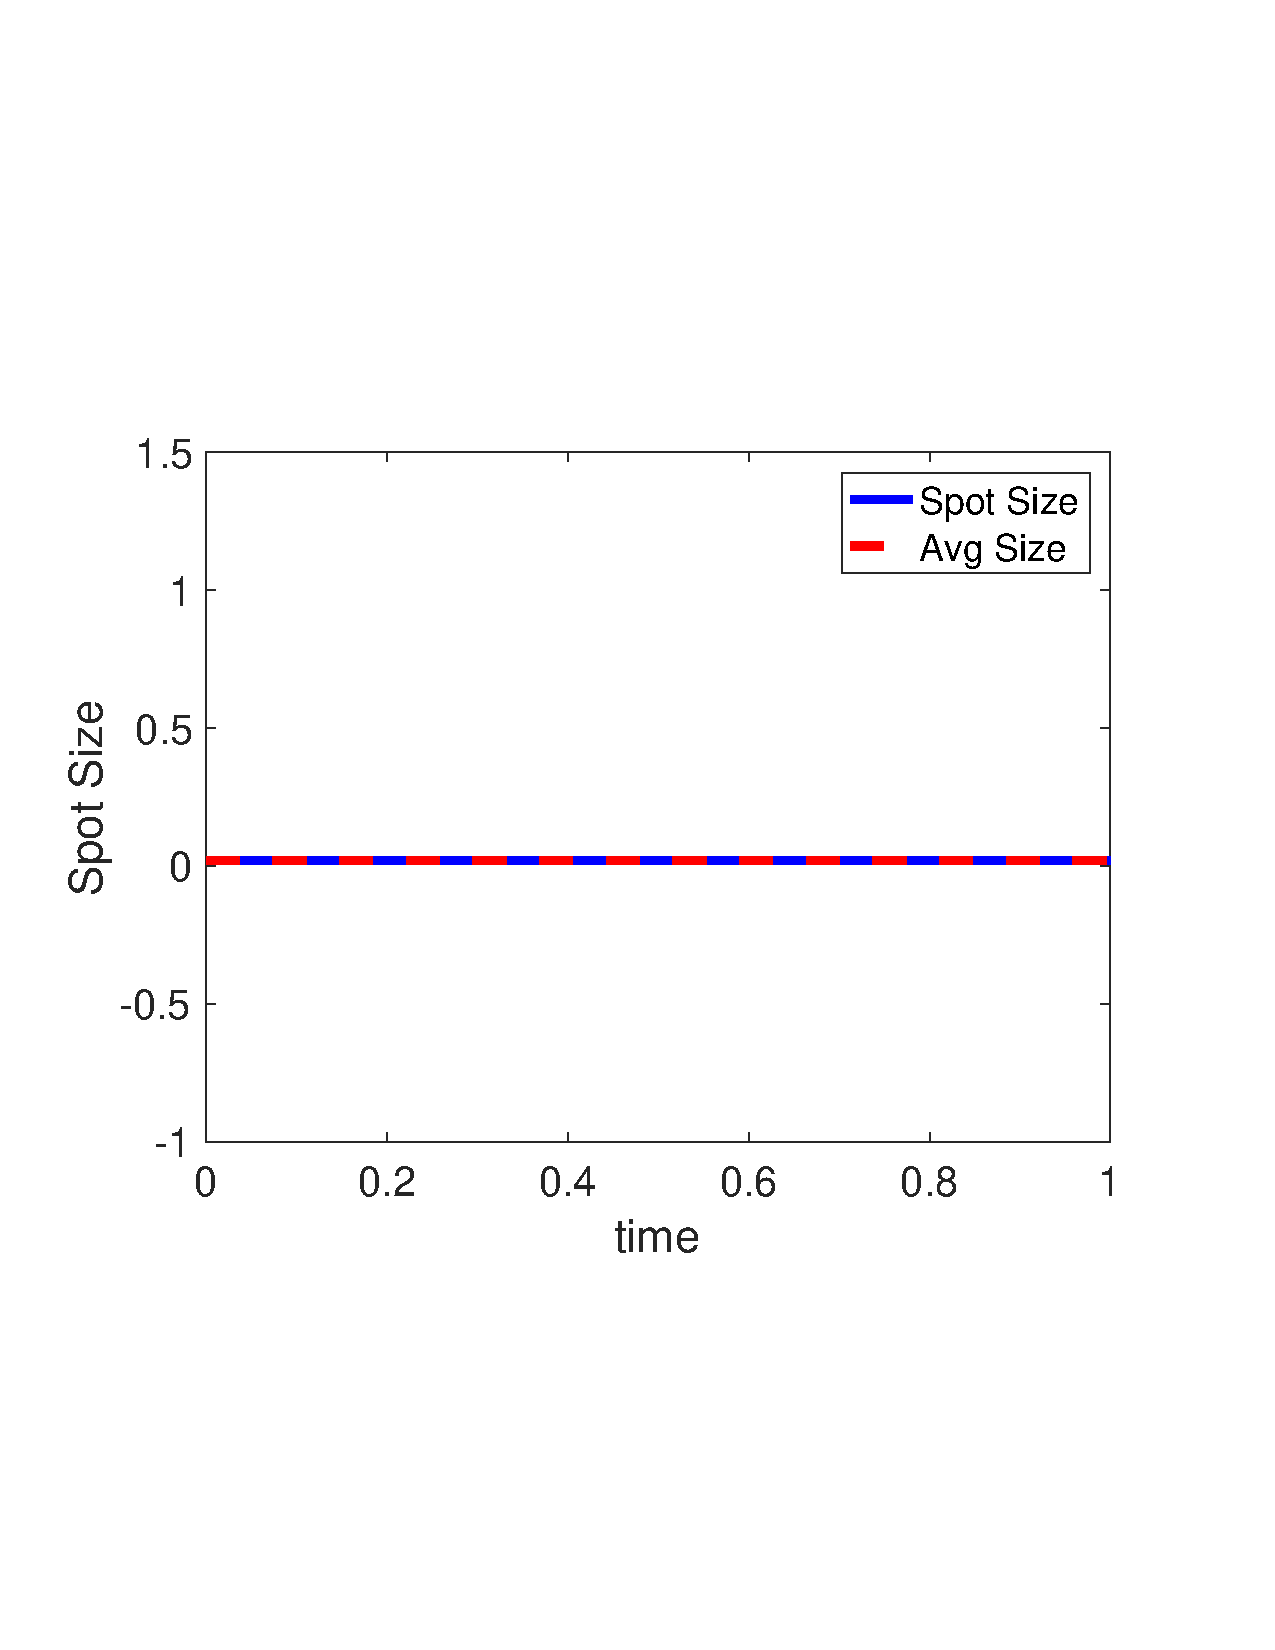
\includegraphics[width=0.65\textwidth,trim=1cm 6cm 2cm 6cm,clip]{Figures/Q5P1_real_SpotSizeEvolution.pdf}
	\caption{Detector plane maximum spot size radius evolution for a single realization.}
	\label{ssEvolution}
\end{figure}


MCS with random input disturbance realizations generate a sufficient number of output data sets for which the distribution parameters, $\mu_{out}$ and $\sigma_{out}$, are computed. These output distributions are then generated for varied user-supplied values of the input distribution parameters, $r_0$ and $\sigma_0$. Figures~\ref{distrel} are plots of the input to output statistics relationships. Analysis of these plots validates some intuition regarding the simulation. Figure~\ref{mu_v_r0} reveals a linear increase in the mean of the average spot size as the mean strength of the input disturbance is increased. Naturally, a larger disturbance generates a greater misalignment and poorer optical performance. Similarly, Figure~\ref{sigma_v_r0} shows a linear increase in the mean of input disturbance promotes an increase in the standard deviation of the average spot size. Figure~\ref{mu_v_sigma0} indicates that an increase in the standard deviation of the input disturbance does not noticeably change the mean of the average spot size except for zero-mean input. This observation suggests that the assumption of a Gaussian distribution of the output is appropriate because the distribution about the mean input mimics to the distribution about the mean output. Figure~\ref{sigma_v_sigma0} reveals an expected result in that the standard deviation about the mean output increases with the standard deviation of the input disturbance. \\

\begin{figure}
	\centering
	\subfigure[]{
	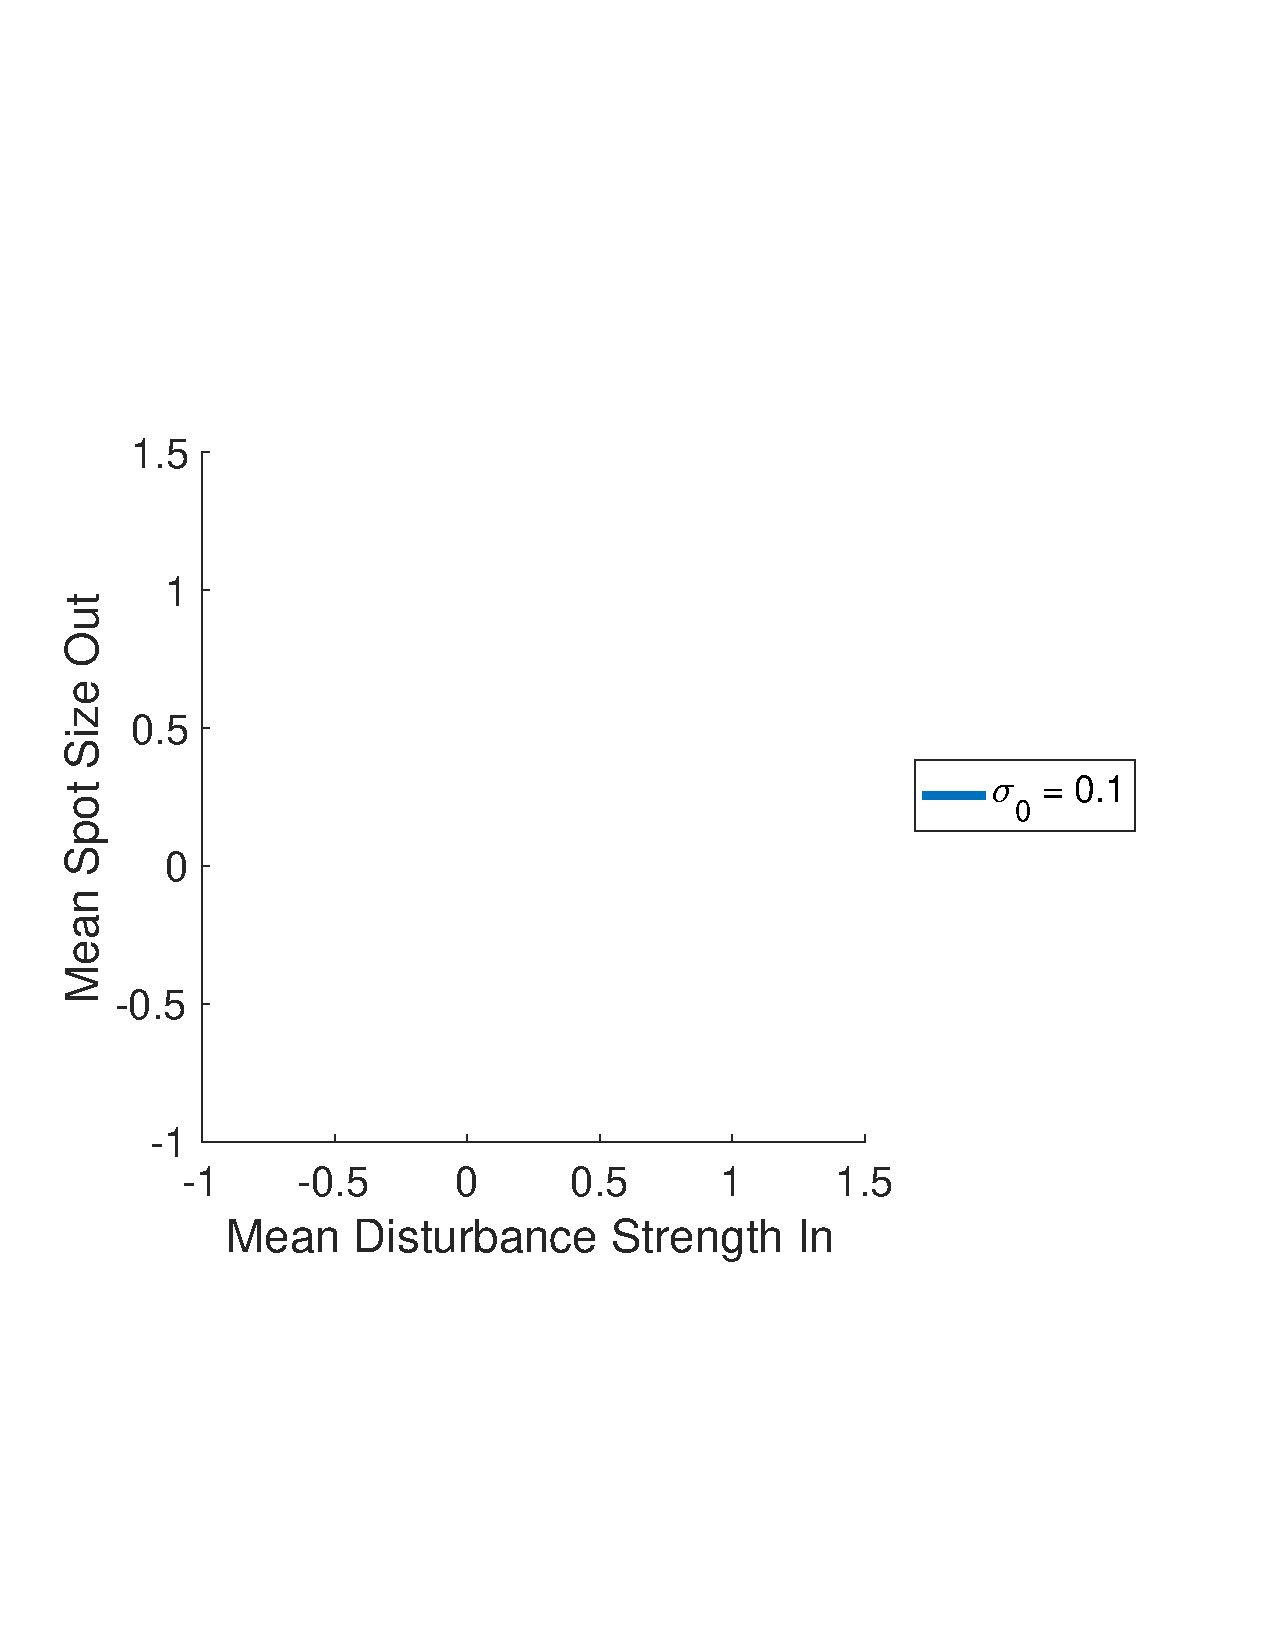
\includegraphics[width=0.45\textwidth,trim=0.8cm 6cm 2cm 6cm,clip]{Figures/Q5P1_stat_mu_v_r0.pdf}
	\label{mu_v_r0}}
	\subfigure[]{
	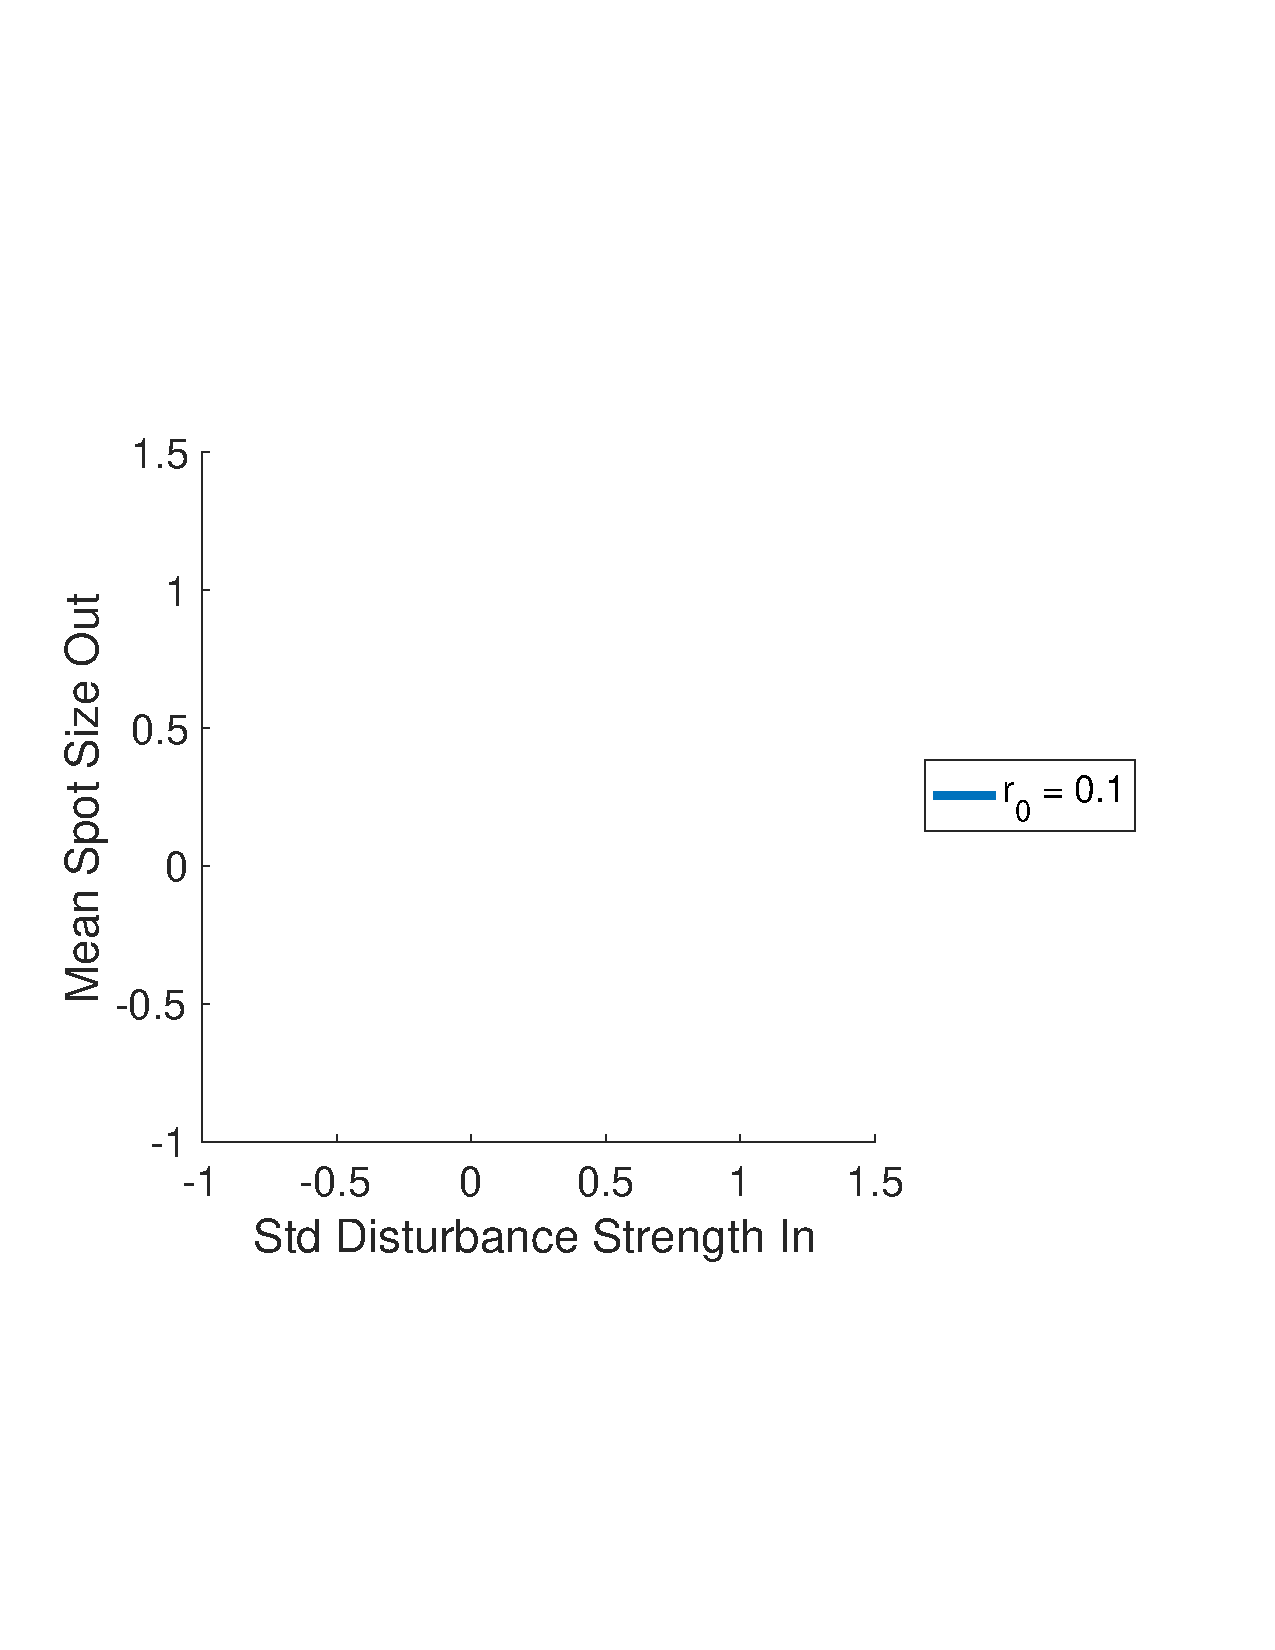
\includegraphics[width=0.45\textwidth,trim=0.8cm 6cm 2cm 6cm,clip]{Figures/Q5P1_stat_mu_v_sigma0.pdf}
	\label{mu_v_sigma0}}
	\subfigure[]{
	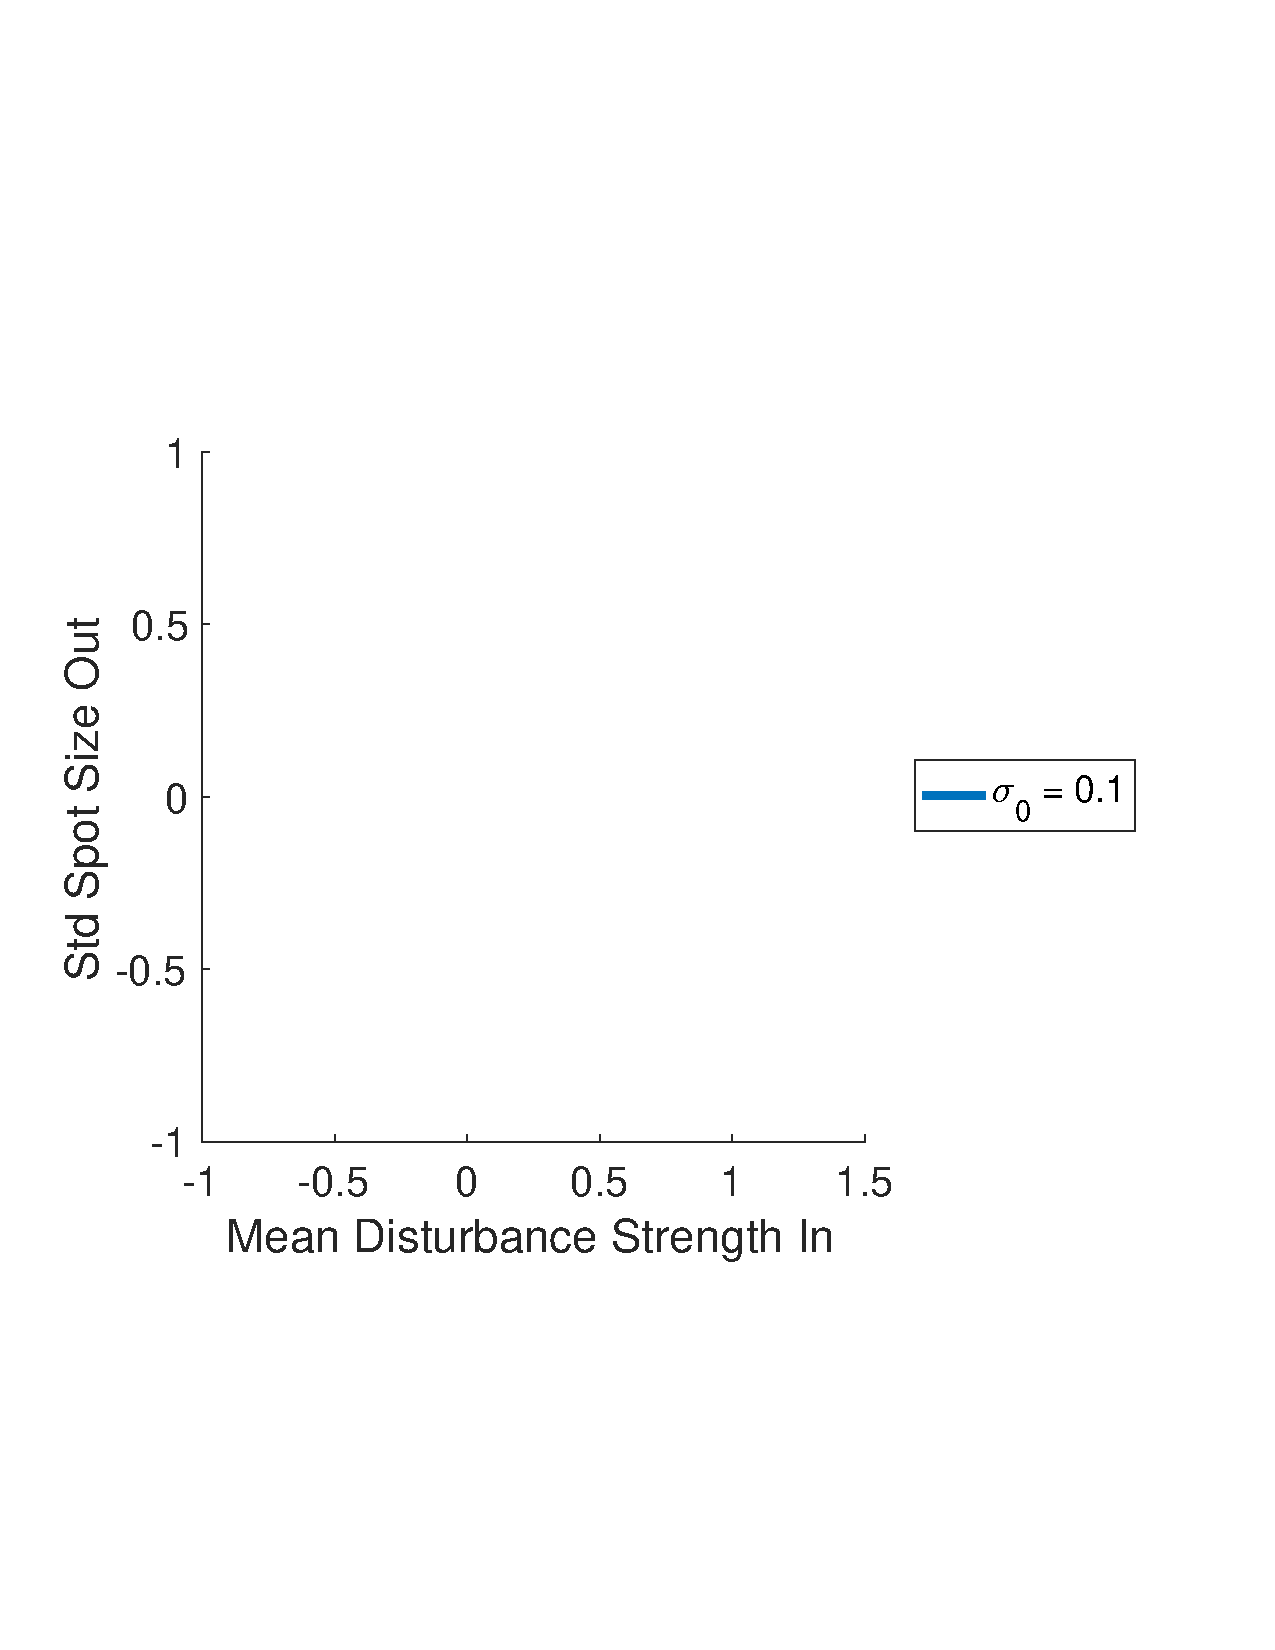
\includegraphics[width=0.45\textwidth,trim=0.8cm 6cm 2cm 6cm,clip]{Figures/Q5P1_stat_sigma_v_r0.pdf}
	\label{sigma_v_r0}}
	\subfigure[]{
	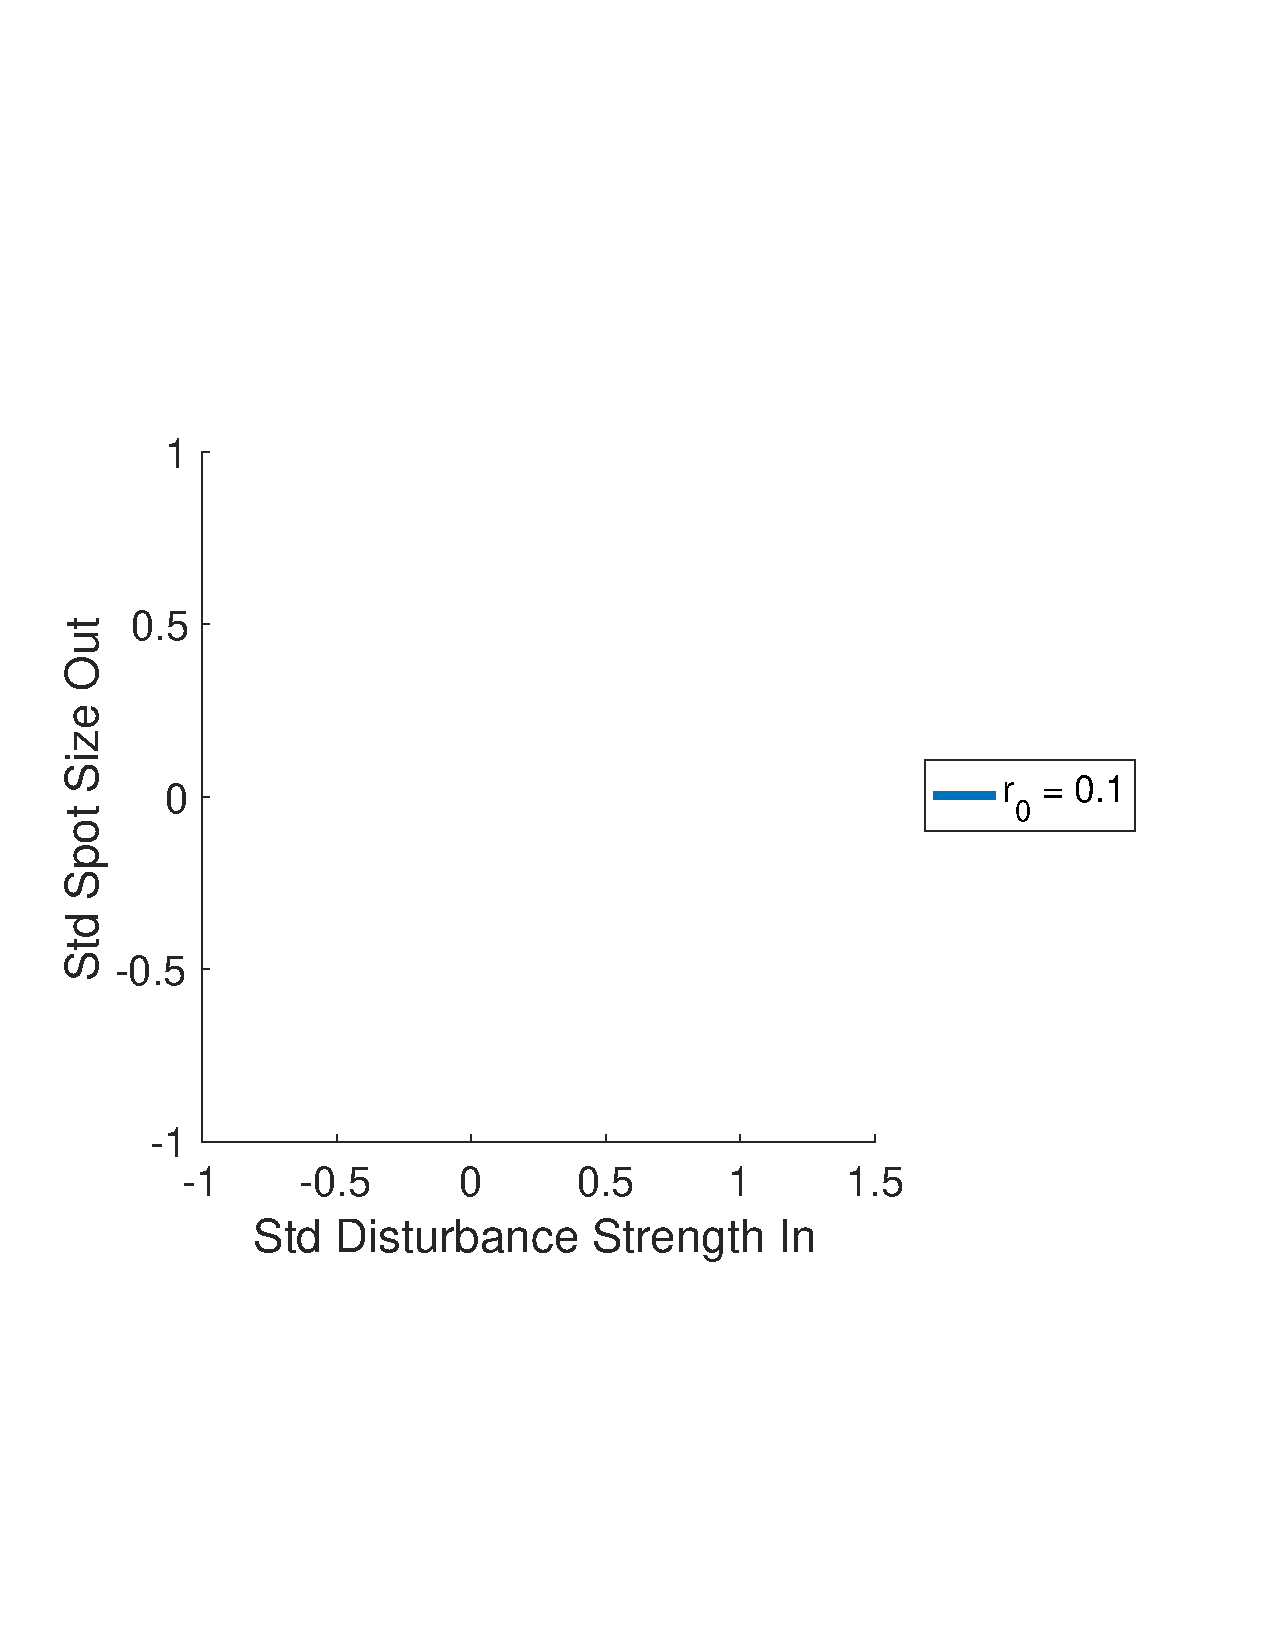
\includegraphics[width=0.45\textwidth,trim=0.8cm 6cm 2cm 6cm,clip]{Figures/Q5P1_stat_sigma_v_sigma0.pdf}
	\label{sigma_v_sigma0}}
	\caption{Distribution parameter relationships}
	\label{distrel}
\end{figure}


\input{6-conclusion}
\bibliographystyle{aiaa}
\bibliography{ref}
\end{document}
